\chapter{Technologischer Aspekt}\label{K3} % For referencing the chapter elsewhere, use \ref{K3} 
\begin{sloppypar}
Zur theoretischen Ausarbeitung gehört die Darstellung der technologischen Aspekte. Im Folgenden soll daher ein Überblick über den Stand der Sprach- und Translationstechnologien gegeben werden. In einem ersten Teil werden die einzelnen Technologien vor dem historischen Hintergrund (folgender Abschnitt \ref{K3:sec:Geschichte-Technologie}) kurz vorgestellt und ausdifferenziert. Konkret geht es um die Unterscheidung zwischen maschineller Übersetzung und Verdolmetschung (Abschnitte \ref{K3:subsec:DiffTech}, S.\,\pageref{K3:subsec:DiffTech} und \ref{K3:sec:CATCAI}, S.\,\pageref{K3:sec:CATCAI}). Ein zweiter Teil (Abschnitt \ref{K3:sec:Qualitaet}, S.\,\pageref{K3:sec:Qualitaet}) geht dann auf die Evaluationsmöglichkeiten ein, die zur Bewertung der Qualität angewendet werden. Damit verbunden ist auch das Postediting sowie die Usability (Abschnitte \ref{K3:sec:PE}, S.\,\pageref{K3:sec:PE} und \ref{K3:sec:Usability}, S.\,\pageref{K3:sec:Usability}).
\end{sloppypar}
%---------------------------------------------------------------------------------------

% Hier müssen noch Dinge wie HQHAMT und HQMAHT erwähnt werden. Ggf. kurzer Abriss der MT Geschichte. Insgesamt nicht mehr als 0,5-1 Seite.

\section{Geschichtlicher Überblick der Technologie}

\label{K3:sec:Geschichte-Technologie}

%---------------------------------------------------------------


Die Entwicklung des Computers in den 1930er und 1940er Jahren wird gemeinhin als Beginn der Forschung zu Sprachtechnologien betrachtet. Was die Betrachtung vom Standpunkt der mechanischen bzw. maschinellen Verarbeitung von natürlicher Sprache angeht, so kann das Aufkommen des Computers als Wegpunkt entlang einer Geschichte, die bereits früher begann, verstanden werden. Sowohl \citet[5]{stein_machine_2013} als auch \citet[431, 434]{hutchins_machine_1995} weisen zu Beginn ihrer Beiträge darauf hin, dass die aktuelle Entwicklung auf diesem Gebiet ohne die früheren Überlegungen nicht zu verstehen ist. Da diese Arbeit jedoch einen hohen technologischen Anteil besitzt, soll die Entwicklung des Computers als definitorischer Ausgangspunkt genügen. Zeitlich vorausgehende Ansätze seien an dieser Stelle demnach nur kurz erwähnt.

\subsection{Bis zum 2.\,Weltkrieg}
\label{K3:para:2WK}

\citet[5]{stein_machine_2013} führt den katalanischen Philosophen Ramon Llull (13. Jahrhundert)\ia{Llull, Ramon} und den deutschen Philosophen Gottfried Wilhelm Leibniz\ia{Leibniz, Gottfried W.} (17. Jahrhundert) als Vordenker an, deren Beiträge zur maschinellen Übersetzung sich vor allem auf dem Gebiet der Universalsprache verorten lassen. Weiter ist der Alchemist Johann Joachim Becher\ia{Becher, Johann Joachim} (17. Jahrhundert) aufgeführt, dessen Überlegungen sich in erster Linie auf die Konzeption eines mechanischen Wörterbuches stützten, das in der Lage war, lateinische Wörter zu kodieren \citep[5]{stein_machine_2013}.

\begin{sloppypar}
Erste praktische Umsetzungen im Bereich der maschinellen Sprachverarbeitung wurden durch den Franzosen George Artsrouni\ia{Artsrouni, George} und den Russen Petr Petrovich Smirnov-Troyanskii\ia{Smirnov-Troyanskii, Petr Petrovich} allerdings erst in den 1930er Jahren unabhängig voneinander ausgearbeitet. Artsrouni konzipierte ein Art Lochkartensystem, das zur Eingabe die passende Übersetzung, sprich: die passende Perforation, auf einem mit Ausgangsbegriff und Übersetzung beschrifteten Papierstreifen suchte. Smir\-nov-Troy\-ans\-kiis Vorhaben umfasste eine dreiphasige Übersetzung. Zunächst sollte ein Mensch, der nur die Ausgangssprache beherrschte, den Ausgangstext in eine von der Maschine verarbeitbare Form bringen, die lediglich eine von Troyanskii entwickelte Symbolsprache und die Grundformen der Wörter im Text umfasste. In der zweiten Phase wandelte die Maschine die in der Symbolsprache kodierten Informationen in die Zielsprache um. Ein Posteditor, der nur die Zielsprache beherrschte, wandelte diese Kodierung im dritten Schritt wieder in eine korrekte sprachliche Form um \citep[434]{hutchins_machine_1995}.\end{sloppypar}

Während des 2.\,Weltkriegs verlagerte sich das Forschungsinteresse auf diesem Gebiet weg von der Übertragung von Informationen von einer in die andere Sprache hin zur Kryptologie. Dabei hat das britische Vorhaben um den Mathematiker Alan Turing\ia{Turing, Alan} bis heute Symbolcharakter, der die Funktionsweise der deutschen Dechiffriermaschine \emph{ENIGMA}\is{ENIGMA} zu verstehen versuchte \citep[6]{stein_machine_2013}.

\subsection{Ab 1946}
\label{K3:para:ab1946}
\begin{sloppypar}
Das Jahr 1946 stellt ein Schlüsseldatum dar. Mit Ende des Weltkriegs richtete sich die Aufmerksamkeit dieses Forschungsbereiches wieder auf die maschinelle Übersetzbarkeit von natürlicher Sprache. Als Ursprung gilt der Schriftverkehr zwischen Warren Weaver\ia{Weaver, Warren}, Mitglied der Rockefeller Foundation, und A.D. Booth\ia{Booth, Andrew D.}, einem Physiker. Weaver hatte einen Bericht Booths gelesen, in dem dieser über die Möglichkeit sprach, Computer für Übersetzungszwecken zu konzipieren \citep[29]{locke_translation_1956}. Booth selbst beschrieb dies wie folgt:
\end{sloppypar}

\begin{quote}
It arose because, in 1946, various new uses for automatic digital calculating machines were being considered and these ranged from the more obvious applications to problems of mathematics and physics, to philosophical problems such as the mechanization of human thought processes, the playing of games and the translation of language. \citep[88]{booth_history_1958}
\end{quote}


Hieraus entwickelte sich ein reges Forschungsinteresse, das sich zunächst auf Wort-für-Wort-Übersetzungen auf Grundlage eines bilingualen Wörterbuches konzentrierte und Syntax und Morphologie außer Acht ließ. Ziel der Bemühungen sollte zunächst sein, Wissenschaftlern (sprachlichen) Zugang zu Texten ihrer Kollegen aus anderen Ländern zu verschaffen \citep[28]{delavenay_introduction_1960}. Um das Forschungsinteresse weiter zu schüren und gleichzeitig in Kontakt mit Kritikern zu treten, veröffentlichte Weaver\ia{Weaver, Warren} 1947 seine Überlegungen in Form des bis heute berühmten \emph{Weaver Memorandums}\is{Weaver Memorandum}. Die darin enthaltenen Ausführungen veranlassten Forscher überall in den USA, sich intensiv mit der MÜ auseinanderzusetzen. So zählt \citet[30]{locke_translation_1956} folgende zentrale Namen aus jener Zeit auf:


\begin{quote}
At the University of Washington Erwin Reifler looked into the basic semantic equivalents of languages. At the University of California at Los Angeles Victor A. Oswald and Stuart L. Fletcher, Jr., analyzed German syntax and in 1951 published the first paper devoted to machine translation: “Proposals for the Mechanical Resolution of German Syntax Patterns.” At M.I.T. Yehoshua Bar-Hillel began an attempt to identify the universal grammar elements in various languages and also gave some thought to translating idioms.
\end{quote}

\begin{sloppypar}
Besonders der Name Bar-Hillel\ia{Bar-Hillel, Yehoshua} ist einerseits eng mit der Erweiterung des Forschungsstands und andererseits auch mit der kritischen Auseinandersetzung der Möglichkeiten verbunden. Er war 1952 einer der Organisatoren der ersten nationalen Konferenz zu \glqq mechanical translation\grqq{} \citep[29]{delavenay_introduction_1960} überhaupt. Finanziert wurde die Konferenz durch die Rockefeller Foundation. Im Jahre 1956 war er dann auch an der Ausrichtung der ersten internationalen Konferenz auf diesem Gebiet beteiligt. Etwa zeitgleich wurde das bis heute wegweisende \emph{George\-town-Experiment}\is{Georgetown-Experiment!Maschinelle Übersetzung} (1954) durchgeführt, dessen Ausgang als Beleg genommen wurde, dass das Problem der maschinellen Übersetzung beinahe gelöst sei. Im Rahmen dieses Experiments wurden russische Sätze mit einem regelbasierten System ins Englische übertragen \citep[15]{koehn_statistical_2009}. Überhaupt erfährt die Auseinandersetzung mit der MÜ in der Zeit nach dem 2.\,Weltkrieg bis in die 1960er Jahre einen enormen Aufschwung. Begünstigt durch das rege Forschungsinteresse entstehen mehrere beachtete Publikationen und regelmäßig erscheinende Fachmagazine, wie etwa die Zeitschrift \emph{Mechanical Translation} von William Locke\ia{Locke, William N.} und Victor Yngve\ia{Yngve, Victor} oder das Buch \emph{Machine Translation of Languages} von Locke und Booth\ia{Booth, Andrew D.} \citep[30]{delavenay_introduction_1960}.
\end{sloppypar}

\subsection{Der ALPAC-Bericht}
\label{K3:para:alpac}

Zu Beginn der 1960er Jahre musste man dann jedoch feststellen, dass die hohen Ziele und die Hoffnungen, die die MÜ-Forscher hatten, mit dem damaligen Stand der Technologie kaum zu erreichen seien. 1960 hatte Bar-Hillel\ia{Bar-Hillel, Yehoshua} in einem Bericht die technischen und linguistischen Probleme bei der MÜ angemerkt. Besonders den damaligen Anspruch, eine \glqq fully automatic high quality translation (FAHQT)\grqq{} \citep[438]{hutchins_machine_1995} erzielen zu wollen, wies Bar-Hillel\ia{Bar-Hillel, Yehoshua} als für den damaligen Stand utopisch zurück. 1961 veröffentlichte Mortimer Taube mit dem Buch \emph{Computers and Common Sense} eine weitere kritische Auseinandersetzung mit der maschinellen Verarbeitung linguistischer Strukturen \citep[9]{henisz-dostert_machine_1979}. Den härtesten Rückschlag erfuhr das Forschungsgebiet jedoch 1966 mit der Veröffentlichung des bis heute berühmten ALPAC-Berichts\is{ALPAC!Automatic Language Processing Advisory Committee}. Das \emph{Automatic Language Processing Advisory Committee} war bereits 1964 von der \emph{National Academy of Science} zur Evaluierung des gegenwärtigen Forschungsstandes gegründet worden. Kernaussagen des Berichtes waren zum einen die Feststellung, dass es mehr Übersetzer{\textperiodcentered}innen als zu übersetzende Texte gäbe. Zum anderen gab das Expertenkommitee die Einschätzung ab, dass die als Maxime ausgegebene FAHQT grundsätzlich möglich, mit den zur damaligen Zeit zur Verfügung stehenden technologischen Ressourcen jedoch nicht realisierbar sei. Weiterhin wog der ALPAC-Bericht das Kosten-Nutzen"=Verhältnis der MÜ ab. Hierbei wurde festgestellt, dass die MÜ ohne menschliche Postedition zu kostspielig und langwierig sei. Zugleich enthielt der Bericht jedoch auch die Empfehlung, der Linguistik weitere Fördergelder zuzugestehen, vor allem mit der Zielsetzung, die Geschwindigkeit und Qualität zu verbessern und die Kosten zu senken \citep[1--34]{automatic_language_processing_advisory_committee_language_1966}.

Rückblickend hält Hutchins dem entgegen, dass der ALPAC-Bericht\is{ALPAC!Automatic Language Processing Advisory Committee} viel zu unausgewogen und von den Absichten der beteiligten Institutionen gelenkt war.


\begin{quote}

The ALPAC report was widely condemned as narrow, biased and shortsighted. It is true that it failed to recognize, for example, that revision of manually produced translations is essential for high quality, and it was unfair to criticize MT for needing to post-edit output. \citep[439]{hutchins_machine_1995}

\end{quote}


Die Auswirkungen waren verheerend, sodass die Forschung in weiten Teilen der USA und Europas zum Erliegen kam oder zumindest auf die rein praktische Anwendung umgestellt wurde. Im Vordergrund stand nun die Entwicklung von digitalen oder maschinellen Hilfsmitteln, die Übersetzer{\textperiodcentered}innen bei ihrer Tätigkeit unterstützen sollten. Für das folgende Jahrzehnt sollte die MÜ in den USA als kaum zukunftsträchtiges Feld stigmatisiert bleiben \citep[6]{stein_machine_2013}. In Kanada und Europa hingegen blieb das Forschungsinteresse -- besonders in der freien Wirtschaft -- bestehen \citep[439]{hutchins_machine_1995}. Hierbei wurden vor allem extrem spezialisierte Systeme entwickelt, die ein genau abgestecktes terminologisches Feld bearbeiten konnten, was \citet[33]{krenz_maschinelle_2008} als \glqq Subsprachen-Systeme\grqq{} benennen. Als ein prominentes Beispiel wird häufig das \emph{MÉTÉO}-Projekt \is{MÉTÉO} der Universität von Montreal und des kanadischen Umweltministeriums genannt, das Wettervorhersagen aus dem Englischen ins Französische übersetzten sollte \citep[38]{bowker_machine_2019}.

\subsection{Technologische Weiterentwicklung}
\label{K3:para:technologische-weiterentwicklung}

Erst Mitte der 1970er Jahre sollte die MÜ jedoch wieder intensivere Beachtung finden. Mit dem Aufkommen leistungsstärkerer Computer kam es auch zur Gründung neuer Forschungsgruppen auf dem Gebiet der Computerlinguistik und zur Entwicklung kommerzieller Systeme wie etwa \emph{Systran}. Systran\is{Systran} ist bis heute eine der bekanntesten Marken weltweit auf diesem Gebiet und wurde in den 1970er Jahren für das Sprachenpaar Englisch-Russisch von der US-Luftwaffe genutzt und wenig später auch von der Europäischen Kommission eingesetzt \citep[139--142]{hutchins_machine_1995}. Mit \emph{Logos}\is{Logos} und \emph{METAL}\is{METAL} kamen in den 1980er Jahren zudem zwei weitere kommerzielle Systeme auf den Markt \citep[35]{koehn_neural_2020}. Dies geschah zunächst in Form der regelbasierten maschinellen Übersetzung (eng. \emph{rule-based machine translation, RBMT}\is{maschinelle Übersetzung!regelbasierte}, dt. \emph{RBMÜ}, s.\,S.\,\pageref{K3:subsec:RBMT}), die insofern aufwändig zu betreiben war, als ein möglichst umfassender und präziser Fundus an grammatischen und morphosyntaktischen Regeln ausgearbeitet und ein umfangreiches zweisprachiges Wörterbuch bereitgestellt werden musste \citep[7]{stein_machine_2013}. Weiterhin erfuhr das Sprachangebot eine Ausdehnung. Während anfangs Französisch, Deutsch, Englisch und Russisch im Fokus standen, kamen im Laufe der Zeit auch Projekte zur Übersetzung des Chinesischen ins Englische (\emph{CULT})\is{CULT} oder gar zu mehrsprachigen Übersetzungen (\emph{TITUS})\is{TITUS} hinzu \citep[34]{krenz_maschinelle_2008}. Als gemeinsames europäisches Projekt wurde zwischen 1970 und 1994 \emph{EUROTRA}\is{EUROTRA} betrieben, das zwar das eigentliche Ziel \glqq des Aufbaus eines modernen Übersetzungssystems\grqq{} \citep[30]{burchardt_deutsche_2012} verfehlte, dennoch nachhaltig zur Entwicklung der Sprachtechnologieforschung in Europa beitrug.

Mit der weltweit steigenden Menge an zu übersetzenden Texten wuchs zu Beginn der 1980er Jahre auch der Bedarf an maschinellen Übersetzungssystemen. Eine Forschungsgruppe von IBM\is{IBM} unter der Leitung von Peter F. Brown\ia{Brown, Peter F.} rückte die statistische maschinelle Übersetzung\is{maschinelle Übersetzung!statistische} in den Fokus des Interesses \citep[7]{stein_maschinelle_2009}.


\begin{quote}

Binnen kürzester Zeit konzentrierte sich die Mehrheit der Forschungen auf die statistischen Ansätze, mit denen man Erfolge erzielen konnte, die mit denen der etablierten, regelbasierten Systeme\is{maschinelle Übersetzung!regelbasierte} vergleichbar waren -- nur dass man zu deren Erstellung keine 10 Jahre Entwicklungszeit und kein Fachwissen von Linguisten benötigte. Ein paar Tage Zeit und große bilinguale Korpora\is{Korpus!bilinguales} (Bitexte) genügten für einen Prototypen. \citep[7]{stein_maschinelle_2009}

\end{quote}


Neben den großen Computer-Unternehmen investierten einige japanische Unternehmen intensiv in den Sektor, so etwa Mitsubishi mit dem System \emph{MELTRAN}\is{Mitsubishi|see{MELTRAN}}, Sanyo und Toshiba mit \emph{AS-TRANSAC}\is{Sanyo}\is{Toshiba}\is{AS-TRANSAC} oder Fujitsu mit \emph{ATLAS}\is{Fujitsu}\is{ATLAS}. Alle Systeme beschränkten sich jedoch auf die Analyse und Übertragung von morphologischen und syntaktischen Strukturen und bedurften der Nachbearbeitung durch den Menschen \citep[442]{hutchins_machine_1995}.

\citet[443]{hutchins_machine_1995} zählt weiterhin die Untersuchung und Theoriebildung zur Interlingua-Übersetzung\is{Übersetzung!interlingua} (s. S.\,\pageref{K3:item:interlingua}), die Weiterentwicklung der bestehenden Systeme und die Arbeit mit künstlicher Intelligenz\is{Künstliche Intelligenz} als wichtigste Forschungsbereiche der Zeit auf dem Gebiet der MÜ. Dies geschah meist auf Grundlage linguistischer Regeln, weshalb RBMÜ\is{maschinelle Übersetzung!regelbasierte} zu jenem Zeitpunkt der verbreitetste Ansatz der MÜ war. Zu Beginn der 1990er Jahre kam zudem das Forschungsinteresse am maschinengestützten Dolmetschen auf. Das populärste Projekt dieser Zeit stammt mit \emph{Verbmobil}\is{Verbmobil} aus Deutschland. Das Ziel des Vorhabens war die Schaffung eines automatischen Echtzeit-Telefondolmetschsystems, das den jeweiligen Kommunikationsparteien\is{Kommunikation} zwischengeschaltet war \citep[]{wahlster_verbmobil_2000}. Damit einher ging die Auseinandersetzung mit digitaler Spracherkennung und -reproduktion \citep[35]{krenz_maschinelle_2008}.

\subsection{Ausweitung des Produktportfolios}
In den frühen 1990er Jahren wandte sich die Forschung und die Softwareentwicklung den \emph{Computer-Aided Translation Tools} (CAT-Tools) zu. Immer kostengünstigere Heimrechner und die Ausbreitung des Internets rechtfertigten diese Tendenz nicht als Ersatz des menschlichen Übersetzers, sondern vielmehr als Ergänzung und Unterstützung der Tätigkeit, da sie neben der eigentlichen Übersetzungsoberfläche zusätzliche Hilfsmittel wie Terminologiedatenbank, Translation Memory und elektronische Wörterbücher boten (und bieten) \citep[38]{bowker_machine_2019}. Ebenfalls in dieser Zeit stellten Unternehmen erste MÜ-Systeme bereit, die online erreichbar waren, so etwa \emph{Minitel} von Systran (1988), \emph{CompuServe} (1992) und als erstes für alle Internetnutzer{\textperiodcentered}innen kostenfrei verfügbares Angebot \emph{BabelFish} wiederum ebenfalls von Systran und AltaVista (1997).

\subsection{Das neue Jahrtausend}
Die Zeit seit der Jahrtausendwende ist vor allem durch eine rasante Weiterentwicklung der Effizienz und einer Ausweitung der möglichen Sprachenkombinationen geprägt. Durch die Kombination von regelbasierter und statistischer maschineller Übersetzung verbesserte sich seit Anfang der 2000er die Ausgabequalität merklich und wurde zunehmend für professionelle Sprachdienstleister attraktiv.

Das bis heute am weitesten verbreitetste, (kosten-)frei zugängliche MÜ-Sys\-tem ist \emph{Google Translate}. 2006 mit lediglich zwei Sprachen ins Leben gerufen, bietet der Dienst mittlerweile die maschinelle Übersetzung in 103 verschiedene Sprachen. Seit 2016 werden einzelne Sprachen sogar auf Basis der neuronalen maschinellen Übersetzung verarbeitet. Weiterhin können Internetseiten oder -- im Rahmen von Google Lens -- auch Straßenschilder u.\,ä. übersetzt werden lassen.


%----------------------------------------------------------------------------------------
\section{Maschinelle Übersetzung}

\label{K3:sec:MUE}

%----------------------------------------------------------------------------------------

Maschinelle Übersetzungssysteme können grundlegend in zwei große Kategorien eingeteilt werden: \emph{regelbasierte}, die auf Grundlage grammatischer Regelsätze und mehrsprachiger Wörterbücher arbeiten, und \emph{datenbasierte} Systeme, die statistisch-algorithmisch vorgehen. Die Kombination beider zu sog. \emph{hybriden} Systemen ist ein Ansatz, der seit Mitte der 2000er verfolgt wird, um die jeweiligen Stärken der beiden Kategorien zu verbinden. Seit Mitte der 2010er kommen vermehrt \emph{neuronale} Systeme zur Anwendung, die in großen Mengen datenbasiert arbeiten und -- grob umrissen -- die Funktionsweise des menschlichen Gehirns imitieren. Als theoretisches Konzept wird zudem häufig auf sog. \emph{Interlingua-Systeme}\is{Übersetzung!maschinelle} verwiesen. Der Ansatz gründet auf dem syntaktischen Formalismus und dem Versuch, die Bedeutung einer Aussage, eines Satzes oder eines ganzen Textes in einer Tiefenstruktur zu formalisieren, die dann in eine andere Sprache übertragen werden kann \citep[16\psq]{koehn_statistical_2009}.
Mit \citet{hutchins_introduction_1997, wilks_machine_2009, koehn_statistical_2009, koehn_neural_2020} sind über die letzten Jahrzehnte umfassende Werke entstanden, die die Entwicklung aus internationaler Perspektive betrachten. Für eine deutschsprachige Sicht auf die MÜ bestehen mit \citet{laisiepen_grundlagen_1996, ramlow_maschinelle_2009, stein_machine_2013,  porsiel_maschinelle_2017} Werke bereit, die sich einer generellen Übersicht verschrieben haben.



%----------------------------------------------------------------------------------------

\subsection{Regelbasierte Maschinelle Übersetzung}

\label{K3:subsec:RBMT}

%----------------------------------------------------------------------------------------
\begin{sloppypar}
Der simpelste Ansatz zur maschinellen Übersetzung\is{maschinelle Übersetzung!regelbasierte} basiert auf vom Menschen zusammengetragenen Grammatik- und Morphologieregeln. Auch heute noch kommt eine hybride Form aus regelbasiertem und statistischem Vorgehen in Übersetzungssystemen vor. Der regelbasierten maschinellen Übersetzung liegt dabei neben dem Repertoire an Regeln auch ein bilinguales Wörterbuch zugrunde, aus dessen Fundus aus der Ausgangs- in die Zielsprache übersetzt wird. Ein großes Problem bei diesem Ansatz ist die geringe Flexibilität der Übersetzung und die je nach Sprachenpaar stark variierende Qualität. Die Ergebnisse sind häufig unbrauchbar, was auch \citet[647]{carstensen_computerlinguistik_2010} kritisieren: \glqq Die Abhängigkeiten der linguistischen Regeln und die umfassende Behandlung von sprachlichen Ausnahmen führen jedoch immer wieder zu Problemen bei der Robustheit und Wartbarkeit.\grqq{}\end{sloppypar}

\citet[8]{stein_maschinelle_2009} charakterisiert RBMÜ\is{maschinelle Übersetzung!regelbasierte} zunächst als ein dreistufiges System aus \glqq Analyse, Transfer und Synthese (bzw. Generierung)\grqq{}. Diese drei Stufen werden weiterhin nach ihrem Grad an Komplexität in \emph{direkte Übersetzung}\is{Übersetzung!direkte}, \emph{Transferübersetzung}\is{Transferübersetzung} und \emph{Interlingua-Übersetzung}\is{Übersetzung!interlingua} unterschieden \citep[8]{stein_maschinelle_2009}.

\begin{itemize}

	
    \item Die direkte Übersetzung ist als Wort"=für-Wort"=Übersetzung zu verstehen. Im Analyseschritt werden die einzelnen Wörter im Ausgangstext identifiziert und mit den Einträgen im bilingualen Wörterbuch abgeglichen. Die Transfer- und Syntheseprozesse gehen gemeinsam einher. Zunächst erfolgt die Ersetzung der einzelnen Wörter in der Zielsprache und dann ggf. die Anpassung der Wortreihenfolge. Als Vorteile werden die Zeit- und Kosteneffizient angeführt \citep[645\psq]{carstensen_computerlinguistik_2010}.
	
    \item Die Transfer"=Übersetzung kann als eine Erweiterung der direkten Übersetzung angesehen werden. Der Analyse- und Transferprozess umfasst in diesem Fall mehr als den Abgleich mit dem Wörterbuch: Hinzu kommt eine semantische und morpho-syntaktische Analyse (\emph{Parsing}). Die so erhaltenen Informationen ermöglichen die Definition von genaueren Regeln. (\cites[8]{stein_maschinelle_2009}[646]{carstensen_computerlinguistik_2010})
   
  	\item \label{K3:item:interlingua} Der Grundgedanke hinter der Interlingua"=Übersetzung ist die Annahme, jede Sprache habe die gleiche tiefenstrukturelle Kodierung und nur das oberflächliche Erscheinungsbild, sprich: Lexik und Grammatik, seien individuell. \glqq Diese abstrakte universalsprachliche Repräsentation würde dann das Ziel und die Quelle sämtlicher Übersetzungssysteme sein.\grqq{} \citep[8]{stein_maschinelle_2009} Der Ausgangstext würde demnach zunächst auf seine semantischen und syntaktischen Funktionen hin analysiert und dann eine gleichwertige Entsprechung im Zieltext erzeugt.

\end{itemize}


%----------------------------------------------------------------------------------------

\subsection{Statistische Maschinelle Übersetzung}

\label{subsecSMT}

%---------------------------------------------------------------


Im Gegensatz zu dem manuell verfassten Repertoire an Grammatikregeln der RBMÜ ist die Grundvoraussetzung für die statistische maschinelle Übersetzung (eng. \emph{SMT}, dt. \emph{SMÜ}) ein umfangreiches, gepflegtes Parallelkorpus für das zu übersetzende Sprachenpaar, auf dessen Grundlage das System trainiert werden kann. \is{maschinelle Übersetzung!statistische} Ist die Größe dieses Korpus ausreichend, lässt sich das SMÜ-System sogar automatisch erstellen \citep[647]{carstensen_computerlinguistik_2010}. Das Parallelkorpus\is{Parallelkorpus|see{Korpus}} erfordert eine umfassende Vorarbeit seitens der menschlichen Übersetzer{\textperiodcentered}innen, da die Texte in beiden Sprachen zunächst auf Satzebene aligniert, d.\,h.: ihren jeweiligen Entsprechungen in Ausgangs- und Zielsprache zugeordnet werden müssen. Die Alignierung\is{Alignierung} wird in einem weiteren Arbeitsschritt auch auf Wortebene durchgeführt, um die Möglichkeiten zur Übersetzung eines Wortes flexibler zu gestalten. Durch diesen Prozess entsteht ein sog. Trainingskorpus\is{Trainingskorpus|see{Korpus}} und ein zweisprachiges Wörterbuch, das jedoch bislang nur die flektierten Formen und nicht die Lemmata enthält. In diesem Trainingskorpus sind zudem die Wahrscheinlichkeiten aufgeführt, mit denen ein Wort in der Ausgangssprache einem Wort in der Zielsprache entspricht. Diesen sog. probabilistischen Ansatz\is{probabilistischer Ansatz|see{maschinelle Übersetzung}} konkretisiert \citet[6]{koehn_statistical_2009} mit den Worten: \glqq Probabilities are used when we have to deal with events with uncertain outcomes, such as a foreign word that may translate into one of many possible English words.\grqq{} So kann in einem folgenden Schritt ein Wortfolgenlexikon erstellt werden, das auf Grundlage der o.\,g.\ Wahrscheinlichkeiten das Auftreten einzelner Wortfolgen dokumentiert.


\begin{quote}\sloppy
Ausgangspunkt der SMÜ ist also ein großes Korpus humanübersetzter Texte, wenn möglich aus dem intendierten Anwendungsbereich. Wenn das SMÜ-System Dokumente einer Maschinenbau-Firma übersetzen soll, sollte auch das Eingabekorpus aus diesem Bereich stammen. \citep[648]{carstensen_computerlinguistik_2010}
\end{quote}


Die Qualität der Ausgabe bei SMÜ ist also in hohem Maße einerseits von der Menge der Daten im bilingualen Trainingskorpus\is{Korpus!bilinguales}\is{Trainingskorpus|see{Korpus}} und andererseits der Häufigkeit der Wortfolge im monolingualen Sprachenmodell abhängig.

\citet[11]{stein_maschinelle_2009} weist hierbei noch auf eine gängige Differenzierung innerhalb der SMT\is{maschinelle Übersetzung!statistische} hin: \glqq Man unterscheidet allgemein zwischen wortbasierter und phrasenbasierter SMÜ.\grqq{}

\begin{itemize}

\item Wie die Bezeichnung der wortbasierten maschinellen Übersetzung vermuten lässt, wird hierbei zunächst eine rein lexikalische Übersetzung vorgenommen. Im Gegensatz zu wortbasierten Ansätzen\is{wortbasierter Ansatz} bei der RBMÜ\is{maschinelle Übersetzung!regelbasierte} wird hier jedoch nicht immer nur der erstbeste Begriff aus dem bilingualen Wörterbuch verwendet. Auf Grundlage statistischer Daten kann für einen Begriff im Ausgangstext abgewogen werden, welcher Begriff in der Zielsprache die wahrscheinlichste Entsprechung ist \citep[82]{koehn_statistical_2009}. \citet[11]{stein_maschinelle_2009} hält dem jedoch entgegen, dass so zwar die Möglichkeit gegeben sei, einen Begriff mit einer Mehrworteinheit zu übersetzen, umgekehrt jedoch eine Mehrworteinheit Wort für Wort übersetzt und ggf. nicht nach einem einzelnen Begriff gesucht werde. \glqq Jedem Wort in der Quellsprache muss also mindestens ein Wort in der Zielsprache entsprechen.\grqq{} \citep[11]{stein_maschinelle_2009}

\item \citet[127]{koehn_statistical_2009} charakterisiert den phrasenbasierten Ansatz\is{phrasenbasierter Ansatz|see{maschinelle Übersetzung}} als die gegenwärtig beste Möglichkeit zur maschinellen Übersetzung mit den Worten: \glqq The currently best performing statistical machine translation systems are based on phrase-based models: models that translate small word sequences at a time.\grqq{} Ein Ausgangstext wird also nicht Wort für Wort verarbeitet, sondern in größere Einheiten aufgeteilt, die jedoch kleiner sind als ein Satz. Dabei handelt es sich um die \emph{Phrasen}. Als Begründung führt \citet[127]{koehn_statistical_2009} an, dass es zwischen Ausgangs- und Zielsprache häufig Wörter gibt, die sich nicht mit einem Wort allein in die Zielsprache übersetzen lassen. Solche Mehrworteinheiten, zuweilen auch als \emph{n-Gramme} bezeichnet, kann die phrasenbasierte maschinelle Übersetzung\is{phrasenbasierter Ansatz|see{maschinelle Übersetzung}} erfassen. Einen weiteren Vorteil sieht \citet[12]{stein_maschinelle_2009} in der Möglichkeit, \glqq bestimmte Disambiguierungsentscheidungen zu treffen.\grqq{}

\end{itemize}


%----------------------------------------------------------------------------------------

\subsection{Neuronale Maschinelle Übersetzung}

\label{K3:subsec:NMT}

%----------------------------------------------------------------------------------------

\begin{sloppypar}
Die Anwendung von neuronalen Netzwerken zur maschinellen Übersetzungen\is{maschinelle Übersetzung!neuronale} ist der jüngste und gegenwärtig am intensivsten untersuchte Bereich in der Sprachtechnologieforschung. So beschrieb ein Beitrag in der Ausgabe 01/17 des MDÜ diesen Ansatz als nächsten \glqq Hype bei der maschinellen Übersetzung\grqq{} \citep[38]{kruger_von_2017}, nicht zuletzt unter Verweis auf die Ankündigung von Google\is{Google}, die 2016 die neuronale maschinelle Übersetzung (eng. \emph{NMT}, dt. \emph{NMÜ}) in den Übersetzungsdienst des Konzerns eingebunden zu haben.\end{sloppypar}

\begin{quote}

Die Ankündigung wurde begleitet von einem wissenschaftlichen Paper, das den ambitioniert klingenden Titel „Bridging the Gap between Human and Machine Translation“ trug. Nicht weniger ambitioniert waren die Behauptungen, die Google in diesem Paper aufstellte. So könnten Evaluatoren stellenweise kaum noch Unterschiede zwischen menschlichen Übersetzern und der Google-NMÜ feststellen, [...]. \citep[38]{kruger_von_2017}

\end{quote}

Bevor jedoch auf die Funktionsweise der NMÜ\is{maschinelle Übersetzung!neuronale} eingegangen werden kann, sollte eine Erklärung zu künstlichen neuronalen Netzwerken im Allgemeinen erfolgen. Um ihre Funktion (\emph{KNN}, bzw. auf englisch \emph{artificial neural network, ANN}\is{Netzwerk!künstliches neuronales} zu verstehen, wird häufig der Vergleich zu dem neuronalen Netzwerk im Nervensystem eines Lebewesens gezogen. Dort gibt es Zellen, die Informationen in Form von elektrischen und chemischen Impulsen untereinander weiterleiten können, die sog. \emph{Neuronen}. Sie sind über Verbindungen, den \emph{Synapsen}, miteinander verbunden. Je häufiger nun eine bestimmte Neuronenverbindung im Gehirn durch einen Impuls aktiviert wird, um so stärker und leichter wird die Impulsverarbeitung im Folgenden \citep[19\psq]{kriesel_kleiner_2005}. Das neuronale Netzwerk bildet somit \glqq relativ stabile Aktivierungsmuster heraus\grqq{} \citep[38]{kruger_von_2017}, die als Lernprozess des Lebewesens verstanden werden. Der Fluchtreflex eines Tieres, das Sprachen(er)lernen und viele weitere musterhafte Tätigkeiten aktivieren so die immer gleichen Regionen im Nervensystem. So ist es Lebewesen wiederum möglich, unbekannte Sachverhalte aufzunehmen und zu verarbeiten, die den bereits bekannten Mustern ähnlich sind.

\subsubsection{Künstliche neuronale Netze}
\begin{sloppypar}
Das Konzept der zerebralen Vernetzung kann künstlich nachgebildet werden. \figref{K3:fig:einfachesANN} zeigt ein solches künstliches neuronales Netzwerk\is{Netzwerk!künstliches neuronales} (eng. \emph{ANN}, dt. \emph{KNN}). Auch hier gibt es Neuronen, die \citeauthor{kriesel_kleiner_2005} als \glqq simple Recheneinheiten\grqq{} \citep[35]{kriesel_kleiner_2005} beschreibt, die über gerichtete, gewichtete Verbindungen verknüpft sind \citep[35]{kriesel_kleiner_2005}. Diese Verbindungen entsprechen den Synapsen und sind in Abbildung \ref{K3:fig:einfachesANN} als dünne Pfeile dargestellt. Die Neuronen eines KNN sind in Schichten (eng. \emph{layers}) angeordnet. Erfährt dieses Netzwerk nun also eine Eingabe (z.\,B. externe Informationen), nimmt die Eingabeschicht (\emph{input layer}) diese auf und verarbeitet sie zu Signalen, die über die unterschiedlich stark oder schwach gewichteten Verbindungen an die verdeckte Schicht (\emph{hidden layer}) weitergeleitet werden. \glqq Je nach Gewicht [...] der Verbindungen, über die bestimmte Signale übertragen werden, empfängt ein „aufnehmendes“ Neuron diese Signale in abgeschwächter oder verstärkter Form, wodurch sich der Aktivierungsstatus dieses Neurons verändert.\grqq{} \citep[39]{kruger_von_2017} Verändert sich der Aktivierungsstatus ausreichend, sodass ein gewisser Schwellenwert überschritten wird, löst dies die Aktivierung des Neurons in der verdeckten Schicht aus. Dieses Neuron \glqq feuert\grqq{} \citep[38]{kriesel_kleiner_2005} also ein Signal ebenfalls über die gewichteten Verbindungen in abgeschwächter oder verstärkter Form zur Ausgangsschicht (\emph{output layer}). Wird dieser Prozess häufig genug wiederholt, bilden sich die eingangs erwähnten Aktivierungsmuster zwischen den künstlichen Neuronen und Verbindungen heraus. Das Netzwerk lernt also allmählich, \glqq in großen Mengen unstrukturierter Daten komplexe Muster zu erkennen, diese zu klassifizieren und mit anderen Mustern in Verbindung zu setzen.\grqq{} \citep[39]{kruger_von_2017}
\end{sloppypar}


In ihrem Webinar zur neuronalen maschinellen Übersetzung\is{maschinelle Übersetzung!neuronale} vom 21.\,Juni\,2017 wiesen \citeauthor{cattelan_introduction_2017} in diesem Zusammenhang jedoch explizit darauf hin, dass die Vorgänge, die sich innerhalb der verdeckten Schicht abspielen, bislang unerschlossen sind und dass aufgrund der Komplexität dieser Vorgänge auch davon ausgegangen werden kann, dass es in jüngerer Zukunft keine ausführliche Erklärung hierzu geben wird \citep[]{cattelan_introduction_2017}. Außerdem sei darauf hingewiesen, dass Abbildung \ref{K3:fig:einfachesANN} lediglich ein vereinfachtes Netzwerk darstellt. Für eine realitätsnahe Abbildung müssen noch weitere (verdeckte) Schichten und Neuronen hinzugedacht werden, was für Nutzer{\textperiodcentered}innen die Notwendigkeit einer enorm hohen Rechenleistung nach sich zieht \citep[39]{kruger_von_2017}.

\begin{figure}
    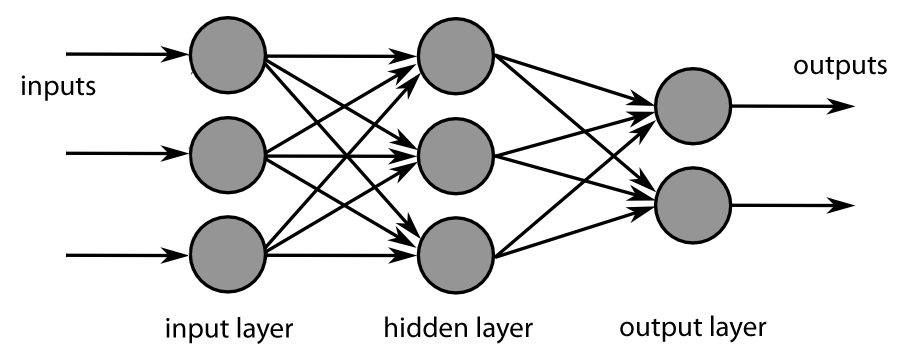
\includegraphics[width=.75\textwidth]{Figures/MultiLayerNeuralNetworkBigger_english.png}
	\caption{Einfaches künstliches neuronales Netzwerk (CC-BY-SA 3.0 H3llkn0wz)\label{K3:fig:einfachesANN}}
\end{figure}

\subsubsection{Ein einfaches Beispiel}

In besagtem Webinar haben \citet{cattelan_introduction_2017} weiterhin die Verarbeitungsprozesse anschaulich am Beispiel einer automatischen Bilderkennung, wie sie auch Google anbietet, erklärt. Aufgabe des Beispielnetzwerkes sollte es sein, eingegebene Bilder einer von vier verschiedenen, stilisierten Tierabbildungen zuzuordnen. Zeigte das eingegebene Bild (\emph{input}) etwa eine Katze, wurden Bildinformationen (Farbwerte, Farbverteilung, Auflösung, usw.) in Zahlenwerte umgewandelt und in das ANN eingespeist (\emph{Signale an der Eingabeschicht}). Anhand dieser Werte konnte das neuronale Netzwerk Aussagen über die am wahrscheinlichsten passende stilisierte Tierabbildung der Eingabe treffen. Durch Eingabe von bislang nicht in dem Bilderkorpus des Beispielnetzwerks enthaltenen Tierfotos kann dann die Präzision trainiert werden \citep[]{cattelan_introduction_2017}. Im Grunde basieren ANN also auch auf einem probabilistischen Ansatz. 

Auf diesem einfachen Beispiel aufbauend lässt sich nun auch die NMÜ erklären. Wie auch bei SMÜ-Systemen ist zunächst ein qualitativ hochwertiges, umfangreiches, bilinguales Textkorpus notwendig. In der Trainingsphase dieses NMÜ-Systems werden nun -- ausgehend von zu Beginn zufälligen Gewichtungen an den Verbindungen der Neuronen -- die Ausgangstexte mit ihren jeweiligen, bereits bekannten Übersetzungen eingegeben. Das ANN ordnet dann anhand von Mustern, die es in den Ausgangstexten identifiziert, passende Zieltexte zu. Nun wird die tatsächliche Ist"=Ausgabe mit der gewünschten Soll"=Ausgabe abgeglichen, wobei der Unterschied zwischen Ist und Soll als Fehler angesehen wird \citep[40]{kruger_von_2017}.

\subsubsection{Backpropagation}

An diesem Punkt gewinnt der sog. \emph{Backpropagation}-Algorithmus an Bedeutung, da er eines der Elemente ist, die dem ANN die Lernfähigkeit überhaupt erst ermöglichen. 


\begin{quote}

When neural networks are used to model a set of existing data so that predictions can be made on new data, the main challenge is to find the set of weight and bias values that generate the outputs that best match the existing data. The most common technique for estimating optimal neural network weights and biases is called back-propagation. \citep{mccaffrey_test_2012}

\end{quote}


Im Bemühen darum, die Differenz zwischen Ist und Soll zu minimieren (und im Optimalfall komplett aufzulösen), überprüft der Algorithmus also stetig die Ausgabe und passt -- gemessen am Goldstandard des Trainingskorpus -- dementsprechend die Gewichtung der einzelnen Verbindungen innerhalb des ANN an. Dieser Vorgang wird so oft wiederholt, bis das ANN die gewünschte Ausgabe liefert \citep[]{habra_neural_2017}.

Für die Nutzung im Umfeld von kleineren Sprachen\footnote{Wobei in diesem Buch jedoch nicht weiter darauf eingegangen wird, was genau \emph{kleine} Sprache bedeutet. Die Definition hängt auch immer vom Kontinent ab, auf dem man sich befindet.} weist Krüger auf die vielversprechenden Forschungsansätze, eine sog. \emph{Zero Shot Translation} zu schaffen. Im konkreten Fall wurde ein NMÜ-System von Google auf die Übersetzung von Texten aus dem Portugiesischen ins Englische und aus dem Englischen ins Spanische trainiert. Danach war dieses System ebenfalls in der Lage, aus dem Portugiesischen ins Spanische zu übersetzen, ohne dafür trainiert worden zu sein \citep[40]{kruger_von_2017}.

\subsubsection{Vektoren}

Diese Beschreibung geht allerdings noch nicht auf einen weiteren wichtigen Prozess ein. Um die Arbeitsschritte eines NMÜ-Systems zu verstehen, fehlt noch eine Erklärung, wie die Texteingabe in Informationen umgewandelt wird, die das Netzwerk verarbeiten kann, um daraus dann erneut einen Zieltext zu erzeugen. Ausgangspunkt hierfür ist zunächst die Aussage von \citet[2]{bahdanau_neural_2017}: 


\begin{quote} 

This neural machine translation approach typically consists of two components, the first of which encodes a source sentence x and the second decodes to a target sentence y. For instance, two recurrent neural networks (RNN) were used [...] to encode a variable-length source sentence into a fixed-length vector and to decode the vector into a variable-length target sentence.
\label{K3:quote-vektoren}

\end{quote}


Der Vorgang des Dekodierens und Enkodierens bezieht sich auf die Prozesse, die an der Eingabe- und an der Ausgabeschicht stattfinden. Die Begriffe, auf denen hier der Fokus liegt, sind viel mehr \emph{recurrent} und \emph{vector}. Vektoren fasst \citet[2]{seidel_matrizen_2005} als eine Matrix auf, \glqq die nur aus einer Zeile
\emph{$\overrightarrow{z}$}\textsubscript{i} = (\emph{a}\textsubscript{i1}, \emph{a}\textsubscript{i2}, ..., \emph{a}\textsubscript{in}) (Zeilenvektor) oder nur aus einer Spalte \emph{$\overrightarrow{s}$}\textsubscript{k} = (\emph{a}\textsubscript{1k}, \emph{a}\textsubscript{2k}, ..., \emph{a}\textsubscript{mk})
(Spaltenvektor) besteht.\grqq

Matrix definiert \citet[1]{seidel_matrizen_2005} als \glqq eine Tabelle, die in Zeilen und Spalten unterteilt ist. Die Einträge in der Matrix lassen sich über die Koordinaten aus Zeilen und Spalten mit den Indizes \emph{m} und \emph{n} direkt ansprechen.\grqq

Damit wird verständlich, was \citet[51]{kriesel_kleiner_2005} meint, wenn er den Eingabevektor (respektiv auch Ausgabevektor) definiert mit den Worten: 


\begin{quote}
Ein Netz mit \emph{n} vielen Eingabeneuronen benötigt \emph{n} Eingaben \emph{x}\textsubscript{1},  \emph{x}\textsubscript{2},  \ldots, \emph{x}\textsubscript{n}. Wir fassen diese als Eingabevektor \emph{x} = (\emph{x}\textsubscript{1},  \emph{x}\textsubscript{2},  \ldots, \emph{x}\textsubscript{n}) auf. Die Eingabedimension bezeichnen wir also mit \emph{n}. Daten werden in ein Neuronales Netz eingegeben, indem die Komponenten des Eingabevektors einfach bei den Eingabeneuronen als Netzeingabe verwendet werden.
\end{quote}


Dies eröffnet dem NMÜ-System die Möglichkeit, \glqq semantische und grammatikalische Relationen zwischen diesen Wörtern\grqq{} \citep[40]{kruger_von_2017} im Vektorraum anhand ihrer Nähe oder Distanz zu erfassen. Je näher die Wörter zueinander stehen, um so ähnlicher sind sie. Diese Relationen werden auch \emph{word embeddings} genannt und werden in einer Tabelle abgelegt, auf die dann wiederum das NMÜ-System zurückgreift \citep[40]{kruger_von_2017}. 

\subsubsection{Rekurrenz}

Neben Vektoren war in dem Zitat von \citeauthor{bahdanau_neural_2017} (S.\,\pageref{K3:quote-vektoren}) die Rede von rekurrenten neuronalen Netzwerken, (eng. \emph{recurrent neural networks}, \emph{RNN}). Durch die Rekurrenz erhält das Netzwerk die Fähigkeit, \glqq die Outputs der Neuronen einer Schicht wieder als neue Inputs in das Netz\grqq{} \citep[41]{kruger_von_2017} einzuspeisen. So können Sprachdaten verarbeitet werden. \citet{cattelan_introduction_2017} skizzierten diesen Prozess folgendermaßen: Signale werden einerseits von einer zur nächsten Schicht weitergeleitet, zugleich jedoch als erneuter Input an einen Zwischenspeicher der vorherigen Schicht zurückgeführt, usw.
So ist es in Bezug auf Sprachdaten dem RNN möglich, den Kontext eines eingegebenen Textes zu erfassen und ausgehend von den einzelnen Einheiten eines Satzes darauf aufbauende Übersetzungen zu generieren.


%----------------------------------------------------------------------------------------

\subsection{Leistungsmerkmale der Systeme}\label{K3:subsec:LeistungSystemeMT}

%----------------------------------------------------------------------------------------
\begin{sloppypar}
Die hier aufgeführten maschinellen Übersetzungssysteme zeichnen sich durch charakteristische Stärken und Schwächen aus. Ganz allgemein weist \citet[20]{koehn_statistical_2009} zunächst darauf hin, dass die maschinelle Übersetzung nicht perfekt sein muss, um einen Nutzen für den Anwender darzustellen. Mit dieser Bemerkung betritt er das Feld des \emph{information retrieval} bzw. der Informationsextraktion. Ausgerichtet am Leitgedanken, generell Verständnis zu schaffen, kann der Nutzen der MÜ in drei Bereiche unterteilt werden: \emph{Assimilation}, \emph{Dissemination} und \emph{Kommunikation}. Erstes Konzept versteht die MÜ als Möglichkeit, fremdsprachliche Inhalte in einer anderen Sprache verfügbar zu machen. Zweiter Begriff verweist auf die Verbreitung von übersetzten Inhalten zwecks Publikation und letztgenannter Begriff dient dem zwischenmenschlichen Austasch in Form von Mails, Chats und ähnlichen eher informell ausgerichteten Bereichen \citep[20]{koehn_statistical_2009}. Gerade letzter Aspekt ist auch mit Blick auf den Skype Translator ein wertvoller Hinweis.
\end{sloppypar}


Die Stärke der RBMÜ liegt dank der notwendigen Wörterbücher als Datengrundlage auf der hohen Terminologiekonsistenz. Allerdings stoßen die Gram\-ma\-tik- und Syntaxregeln auch bei noch so minutiöser Ausarbeitung bei Sprachen mit offenen Satzstrukturen rasch an ihre Grenzen, sodass die Ausgabe je nach Domäne und Sprachkombination nur schwer leserlich und fehlerbehaftet ist. Russisch, Baskisch oder Türkisch stellen RBMÜ-Systeme beispielsweise regelmäßig vor größte Herausforderungen.

Die SMÜ produziert zwar demgegenüber eine besser lesbare Ausgabe, jedoch bedarf es eines umfassenden Trainings auf Basis eines sauberen zweisprachigen Goldstandard-Korpus' \citep[44]{bowker_machine_2019}. Je domänenspezifischer die Anpassung des Systems ist, desto genauere Ergebnisse produziert die SMÜ. 

Die neuronale MÜ machte in jüngster Zeit besonders von sich reden. Mehrere Publikationen suggerierten auf Grundlage einzelner neuronal übersetzter Beispieltexte einen Abgesang auf die Übersetzung durch den Menschen. Mildere Prognosen sehen zumindest eine erhebliche Konkurrenzsituation für die Übersetzungsbranche, da die gestesteten Systeme schnell, flüssig und kosteneffizient Ergebnisse liefern, die für einen Laien durchaus brauchbar erscheinen.\footnote{Vgl. hierzu beispielsweise die Beiträge von \citet{holzki_digitale_2020, himmelein_smarte_2019}.} Die NMÜ zeichnet sich vor allem durch eine gute Verarbeitung offener Satzstrukturen aus und erweitert sich durch jede Eingabe selbstständig (Schlagwort: \emph{machine learning}) \citep[45]{bowker_machine_2019}. Allerdings ist die NMÜ auch die ressourcenaufwändigste Variante, da die neuronalen Netze auf Grundlage großer mehrsprachiger Korpora gewichtet werden müssen und allein dieser Prozess rechenintensiv ist. Weiterhin führen unbekannte Lexeme und Realia zu Auslassungen von z.\,T. ganzen Phrasen oder gar Sätzen in der Ausgabe. Ein ebenso schwerwiegendes Defizit ist die Invertierung des Sinns einer Aussage. Diese Bereiche problematisiert auch \citeauthor{koehn_neural_2020} mehrfach: Bei der Aufbereitung der notwendigen Textquellen ist auf das jeweilige Urheberrecht zu achten \citep[7]{koehn_neural_2020}. Sprachenpaarabhängige Probleme in Bezug auf Lexik, Semantik und Syntax sind individuell zu betrachten \citep[9]{koehn_neural_2020}. Die maschinelle Übersetzung kann manche realweltliche Probleme schlichtweg nicht erkennen, lösen und übersetzen. Nicht zuletzt bedarf es für einen sinnvollen Einsatz von MÜ im professionellen Kontext eines domänenspezifischen Trainings, was erneut viel Zeit und Ressourcen erfordert. Gerade an diesem Punkt werde es sogar für Sprachdienstleister in puncto Ausstattung und Fachkenntnissen schwierig, allen Erfordernissen nachzukommen \citep[22]{koehn_neural_2020}.


%----------------------------------------------------------------------------------------

\section{CAT und CAI}\label{K3:sec:CATCAI}

%----------------------------------------------------------------------------------------

Wie eingangs (s. S.\,\pageref{K3}) bereits erwähnt, soll sich an dieser Stelle nur eine kurze Darstellung der Systeme zur computerbasierten Unterstützung von Übersetzer{\textperiodcentered}innen und Dolmetschern finden. Computerunterstützte Übersetzungs- und Dolmetschsysteme (jeweils \emph{CAT}- und \emph{CAI}-Tools) stehen dem Anwender unterstützend bei seiner Tätigkeit zur Hilfe, verarbeiten die Eingabe jedoch -- im Gegensatz zu den vorausgehend beschriebenen MÜ-Systemen -- nicht vollautomatisch. Die Grenzziehung an dieser Stelle scheint sinnvoll, da sich CAT- und CAI-Systeme offensichtlich am Randbereich der maschinellen Übersetzung befinden. 

So zählt sie \citet[244]{zimmermann_maschinelle_2012} beispielsweise nur \glqq [i]m weiteren Sinne\grqq{} dazu und \citet[642, 654]{carstensen_computerlinguistik_2010} widmen den Systemen zwar ein Unterkapitel, unterscheiden übergeordnet jedoch explizit zwischen maschineller und computergestützter Übersetzung. Ganz klar unterscheidet \citet[431]{hutchins_machine_1995} zwischen MÜ und CAT- bzw. CAI-Tools mit den Worten: \glqq It excludes computer-based translation tools which support translators by providing access to on-line dictionaries, remote terminology databanks, transmission and reception of texts, etc.\grqq{} Auch wenn er im Folgenden ebenfalls darauf hinweist, dass sich entlang dieser Grenze viele Gemeinsamkeiten finden lassen \citep[431]{hutchins_machine_1995}.

\begin{sloppypar}
\citet[4]{bowker_computer-aided_2002} nimmt an dieser Stelle ebenfalls eine klare Unterscheidung vor, die sie mit Verweis auf die bestehende Terminologie der \emph{human-assisted machine translation} ({HAMT}) und der \emph{machine-assisted human translation} ({MAHT}) verdeutlicht. Diese zwei Begriffe sieht sie als Standard, die weithin als MÜ und CAT bekannt sind. Als Unterscheidungsmerkmal dient ihr vor allem die Verantwortung (wobei auf die urheberrechtliche Dimension hierbei nicht weiter eingegangen wird), wer für die Übersetzung zuständig ist. Während bei der MÜ hauptsächlich der Computer die Verarbeitung des Textes vornimmt und lediglich durch Pre- und Postediting vom Menschen begleitet wird, liegt die Verantwortung bei CAT-Systemen durchweg bei menschlichen Übersetzer{\textperiodcentered}innen, deren Arbeitsabläufe durch die Technologie beschleunigt und vereinfacht werden.

Ihre Definition umfasst allerdings auch Hilfsmittel, die möglicherweise zu selbstverständlich im Alltag verankert sind, so etwa die Rechtschreibprüfung und das Internet:
\end{sloppypar}

\begin{quote}
In its broadest definition, CAT technology can be understood to include any type of computerized tool that translators use to help them do their job. This could encompass tools such as word processors, grammar checkers, e-mail, and the World Wide Web (WWW). \citep[6]{bowker_computer-aided_2002}
\end{quote}


\citet[655]{carstensen_computerlinguistik_2010} betrachten hingegen in erster Linie die an die beruflichen Bedürfnisse angepassten Arbeitsumgebungen, Alignierungsprogramme und die Möglichkeit zur Verwaltung von Terminologiedatenbanken als Kernelemente.

\begin{sloppypar}
In diese Richtung tendiert auch \citet[1]{seewald-heeg_einsatz_2005}, die das Wesen von CAT-Tools, neben den bereits o.\,g.\ Hilfsmitteln zur Kommunikation, Textverarbeitung und auch Angebotserstellung, über die \emph{Translation Memory}-Systeme (\emph{TM}) definiert, die vorgenommene Übersetzungen speichern und sie mit dem aktuellen Auftrag abgleichen, sodass Benutzer{\textperiodcentered}innen teilweise (\emph{fuzzy matches}) oder vollständige übereinstimmungen einfach übernehmen können. \citet[246]{zimmermann_maschinelle_2012} erwähnt außerdem noch die Glossarfunktion, mit der die Nachbearbeitung (\emph{Post Editing}) verbessert werden soll. Auch \citet[21\psq]{koehn_neural_2020} verweist in diese Richtung, indem er noch einmal besonders den Mehrwert der NMÜ als jüngstes System in diesem Bereich hervorhebt: Zwar reiche die Qualität der Übersetzung nicht an die einer professionellen, menschlichen Leistung heran, jedoch biete gerade die NMÜ kreative Übersetzungsvorschläge, die ein statistisches oder regelbasiertes System so nicht erwägen würde.
\end{sloppypar}

In Bezug auf das Dolmetschen sind andere Grundvoraussetzungen gegeben, die wiederum andere Ansprüche an die Fähigkeiten der CAI-Tools stellen. So spricht \citet[411]{fantinuoli_interpretbank:_2009} von Dolmetschern als Fachgebietslaien, die sich \glqq auf einen bevorstehenden technischen Einsatz gezielt vorbereiten und sowohl fachliches als auch terminologisches Wissen aneignen\grqq{} müssen. Allerdings bemängelt er die bislang fehlenden technologischen Möglichkeiten, die den Dolmetschern zur Vorbereitung und während der Aufträge zur Verfügung stehen. Während sich allmählich zwar ein Forschungs- und Entwicklungsinteresse in dieser Richtung herausbilden würde, bestünden die gegenwärtigen Werkzeuge eines Übersetzers noch aus Stift, Papier und allenfalls Word und Excel \citep[2]{fantinuoli_interpretbank:_2009}.

Eine Kommunikationsanwendung wie der Skype Translator, der die Nachrichten maschinell übersetzt, ragt also in gewissem Maße in den Bereich der übersetzerischen Hilfsmittel hinein. Welche Merkmale in der Software wiederzufinden sind, zeigt der folgende Abschnitt auf. 

%----------------------------------------------------------------------------------------

\section{Dienste für Voice- und Video-Chat}

\label{K3:sec:Dienste}

% Neben Skype auch Viber, Google Hangouts, Appear.in, Facebook Chat, ICQ

%---------------------------------------------------------------


Skype mag lange Zeit die bekannteste Software für Voice- und Video-Chats gewesen sein. Eine Monopolstellung hat die Anwendung dadurch jedoch nicht mehr. Die Konkurrenten Facebook und Google betreiben jeweils mit ihrem \emph{Facebook Messenger}\is{Facebook!Messenger} und \emph{Google Hangouts}\is{Google!Hangouts}\is{Google Hangouts|see{Google}}\footnote{Die Studie wurde knapp vor der Bekanntgabe durch Google konzipiert, Google Hangouts in seiner damaligen Form abzuschalten und sowohl für Privat- als auch Firmenkunden als \glqq Hangouts Chat\grqq{} anzubieten. Zum Zeitpunkt des Verfassens dieser Arbeit war der Migrationsprozess der Kunden jedoch noch im Gange. Daher wurde der Namen \glqq Google Hangouts\grqq{} weiterhin im Fragebogen belassen. Für die genaueren Hintergründe s.\,z.\,B. \url{https://arstechnica.com/gadgets/2019/01/the-great-google-hangouts-shutdown-begins-october-2019/}, abgerufen am \datum{}.} Anwendungen, die Voice- und Video-Chats unterstützen. Auch Apple bietet mit \emph{Facetime} einen eigenen Dienst in diesem Segment.

Ferner existieren kleinere Dienste wie etwa die Smartphone-App \emph{Viber} oder die browserbasierte Anwendung \emph{appear.in}\footnote{\url{https://www.appear.in}: Offenbar aus rechtlichen Gründen wurde der Dienst umbenannt in \emph{Whereby}, \url{https://whereby.com/}. Während der Ausarbeitung dieses Buches agierte der Dienst jedoch noch unter altem Namen. Beide Links abgerufen am \datum{}.}. In den 2000er Jahren waren zudem die Dienste \emph{ICQ} und der \emph{Microsoft Windows Live Messenger}\is{Microsoft!Windows Live Messenger}\is{MSN|see{Windows}}\is{Windows Live Messenger|see{Microsoft}} beliebte Plattformen für Video- und Voice-, aber vor allem für Textchats. Die meisten Dienste erfordern eine Registrierung und die Erstellung eines Nutzeraccounts. Hierbei werden mitunter personenspezifische Daten wie bevorzugte Sprache, Geschlecht oder das Alter erhoben. Die Angabe ist in den meisten Fällen jedoch freiwillig. Da viele der Programme auch als mobile Version zur Verfügung stehen, wird bei der Anmeldung auch die Handynummer entweder zwingend oder optional erfasst. Nutzungsgebühren fallen bei Verwendung der Standardversionen keine an, jedoch bieten die meisten Dienste erweiterte Funktionen wie Gruppenchats, Add-Ons oder Festnetztelefonie, welche dann wiederum kostenpflichtig sind.

Die Recherche nach verlässlichen Nutzungszahlen gestaltet sich als schwierig, wenn nicht nur auf die firmeneigenen Angaben vertraut werden soll. Oftmals fehlen Angaben zur Nutzungsdauer und -frequenz. Ein weiteres Problem sind die schwankenden Nutzungszahlen nach Region. Einer Datenerhebung von Statista zufolge nutzten im Jahr 2017 etwa 300 Mio. Menschen monatlich den Facebook Messenger\is{Facebook!Messenger} für Voice- und Videochats \citep[]{statista_facebook_2017}.

In enger Verwandtschaft zu diesen Arten der Kommunikationssoftware stehen zweierlei Konzepte, die immer stärker in die Lebenswelt des Menschen drängen. Dabei handelt es sich einerseits um Chat-Bots, also textbasierte Dialogsysteme, die den Nutzer{\textperiodcentered}innen eine menschliche Kommunikation simulieren. Sie werden dort eingesetzt, wo es zu häufigen Anfragen kommt, die wiederum durch einfache Verschlagwortung und das sog. \emph{Information Retrieval} gelöst werden können. Internationale Unternehmen etwa haben auf ihren Webseiten eben diese Chat-Bots implementiert, die ohne die Kosten von menschlichen Sachbearbeitern die Anfragen der Kund{\textperiodcentered}innen kanalisieren und geläufige Probleme beantworten können.

Andererseits wird das Prinzip des Chat-Bots von sog. \emph{Personal Assistants} aufgegriffen, die über die einfache Frage-Antwort-Verarbeitung hinaus auch (Sprach-)\linebreak[3]Befehle der Anwender{\textperiodcentered}innen aufgreifen und ausführen können. Die Paradebeispiele hierfür stammen von den global bekannten Technologiekonzernen Amazon\is{Amazon}, Google\is{Google} und Apple\is{Apple} und sind unter den Namen \emph{Alexa}\is{Amazon!Alexa}\is{Alexa|see{Amazon}}, \emph{Google Assistant} und \emph{Siri}\is{Apple!Siri}\is{Siri|see{Apple}} bekannt. Durch die Installation des physischen Lautsprechers im Haushalt ist es möglich, gekoppelte Geräte im selben Netzwerk zu steuern, Informationen und Nachrichten abzurufen oder gar Bestellungen im Internet zu tätigen.

%----------------------------------------------------------------------------------------

\subsection{Skype}\largerpage

\label{K3:subsec:Skype}

%----------------------------------------------------------------------------------------

Zu Beginn des neuen Jahrtausends war Skype eine Zeit lang die wohl bekannteste Instant-Messaging-Software für Video- und Voice-Chats. 2003 wurde der Dienst von Skype Technologies entwickelt, bevor er 2011 von Microsoft aufgekauft wurde. Die Verwendung des Dienstes bedarf lediglich der Registrierung und Erstellung eines kostenfreien Nutzerkontos. Für die Kommunikation über Skype sind jeweils ein Gerät zur Toneingabe und zur -ausgabe von Nöten. Dabei kann es sich sowohl um ein Headset mit Mikrophon und Köpfhörern als auch um ein separates Mikrophon und Lautsprecher handeln. Der Videochat erfordert eine Webcam. Derzeit steht die Software für die Betriebssysteme MacOS, Windows und Linux zur Verfügung. Darüber hinaus ist sie als App für Android und iOS erhältlich, oder kann plattformunabhängig in ausgewählten Browsern gestartet werden.

Neben den bereits angesprochenen Voice- und Videochats bietet der Dienst eine Konferenzschaltung mit bis zu 25 Personen, Dateienübertragung, Anrufe und SMS (beides kostenpflichtig) auf Festnetz und Mobiltelefon, Bildschirmübertragung und eine Business-Version mit erweiterten Konferenzeinstellungen. Für die vorliegende Monographie ist die Funktion des Skype Translators von zentralem Interesse, die gegenwärtig (Stand: \datum{}) Arabisch, Mandarin, Deutsch, Französisch, Englisch, Italienisch, Japanisch, südamerikanisches Portugiesisch, Russisch und Spanisch für Sprach- und Videoanrufe\footnote{Auf der firmeneigenen Website geht Microsoft nicht auf die einzelnen Sprachvarietäten ein. Daher ist die Aufzählung hier ebenso oberflächlich gehalten.} sowie 60 weitere Sprachen für Textchats unterstützt. Der Skype Translator läuft auf allen gängigen Plattformen ab Windows\,7 sowie auf MacOS X, iOS, Android bzw. Linux. Alternativ lässt sich die Funktion auch in der Browserversion -- dort allerdings nur mit Google Chrome, Safari oder Microsoft Edge -- zuschalten.

Eine Veröffentlichung des Fraunhofer-Instituts für Eingebettete Systeme und Kommunikationstechnik (ESK) aus dem Jahre 2013 beziffert die Nutzer{\textperiodcentered}innen auf insgesamt 650 Mio. weltweit \citep[6]{messerer_einsatz_2013}. Weiterhin beschreibt selbige Publikation die Skype zugrunde liegende Technologie. So handelt es sich bei dem Dienst um ein sog. Peer-to-Peer-System, das die dynamische Erweiterung und Strukturierung des Netzwerkes ermöglicht. Im Gegensatz zu Festnetz- und Mobiltelefonen ist bei Skype keine Notruffunktion vorhanden. Außerdem hängt die Kommunikationsqualität stark von der zur Verfügung stehenden Bandbreite und der Netzwerkauslastung ab \citep[4]{messerer_einsatz_2013}.

Zum Kreis der Nutzer{\textperiodcentered}innen gehören vor allem Privatpersonen. Durch die in jüngerer Zeit implementierten Office-Anwendungen und die Ausweitung der Business-Version bemüht sich Skype jedoch auch verstärkt um Unternehmen.


%----------------------------------------------------------------------------------------

\subsection{Skype Translator}\largerpage
\label{K3:subsec:SkypeTranslator}

%----------------------------------------------------------------------------------------

Die Funktion des Skype Translators konnte in seinem alten Konzept (bis zum 13. Januar 2020) als sog. Chat-Bot während der Kommunikation mit einem Gesprächspartner aufgerufen werden. Mit dem Befehl \emph{\@Skypetranslator languages} ließen sich die zur Verfügung stehenden Sprachen auswählen (Abb. \ref{K3:fig:Browser-Sprachauswahl-ST} auf S.\,\pageref{K3:fig:Browser-Sprachauswahl-ST} zeigt dies z.\,B.\ für die Browser-Version). Seit dem 13. Januar 2020 ist der Skype Translator tiefer in die Chat-Umgebung integriert: Eine Aktivierung ist nicht mehr nötig, der automatische Übersetzungsdienst orientiert sich an der Spracheinstellung des jeweiligen Endgerätes, sodass er aktiv wird, sobald die Spracheinstellungen der beteiligten Parteien voneinander abweichen. Der eingegebene Text wird dann automatisch als Übersetzung ausgegeben, wobei mit einem Klick auf den Schriftzug \emph{Original anzeigen}, der sich unmittelbar unterhalb der Nachricht befindet, auch der ursprüngliche Text betrachtet werden kann.

%------------------------------------------------------
% Browser ST Sprachauswahl

\begin{figure}
    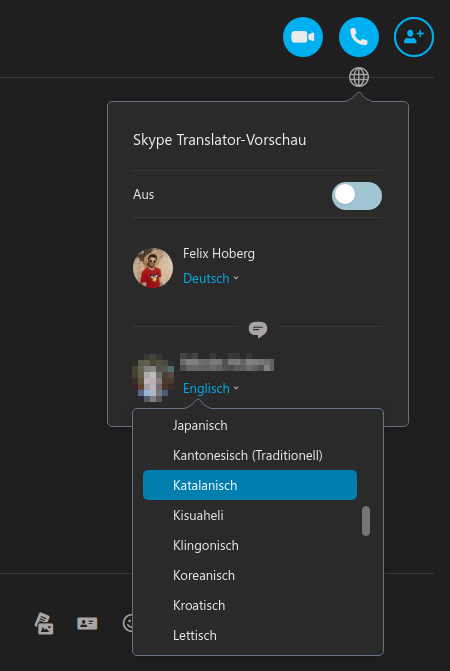
\includegraphics[width=.7\textwidth]{Figures/Skype/browser_skype_translator-ausschnitt.png}
	\caption{Sprachauswahl in der Browserversion des ST\label{K3:fig:Browser-Sprachauswahl-ST}}
\end{figure}

%------------------------------------------------------

Für die weitere Betrachtung des Skype Translators ist der Hinweis wichtig, dass das Chatfenster keinen automatischen Zeilenumbruch besitzt. Mit Chatfenster ist im Folgenden der Bereich gemeint, in dem die Chatbeiträge auf dem Bildschirm angezeigt werden. Zwar verfügt die Desktopanwendung ebenso wie die Browser-Version über \emph{responsive design}, sprich: die Größe und Anordnung der Textnachrichten sowie das generelle Layout werden auf Grundlage der Bildschirmgröße proportional skaliert, jedoch kann es je nach Nachrichtenlänge dennoch zu Überlappungen der beiden Bereiche für ein- und ausgehende Nachrichten kommen (s. \figref{K3:fig:Ausschnitt-Ausgabe-MT-ST}, S.\,\pageref{K3:fig:Ausschnitt-Ausgabe-MT-ST}). Eine ausführliche Diskussion dieses Aufbaus findet in den Abschnitten \ref{K5:subsubsec:DynAOI} (S.\,\pageref{K5:subsubsec:DynAOI}), \ref{K6:sub:catde:graph-inspect} (S.\,\pageref{K6:sub:catde:graph-inspect}) sowie \ref{K6:sub:dede:graph-inspect} (S.\,\pageref{K6:sub:dede:graph-inspect}) statt.

%------------------------------------------------------
% Ausschnitt MT ST

\begin{figure}
    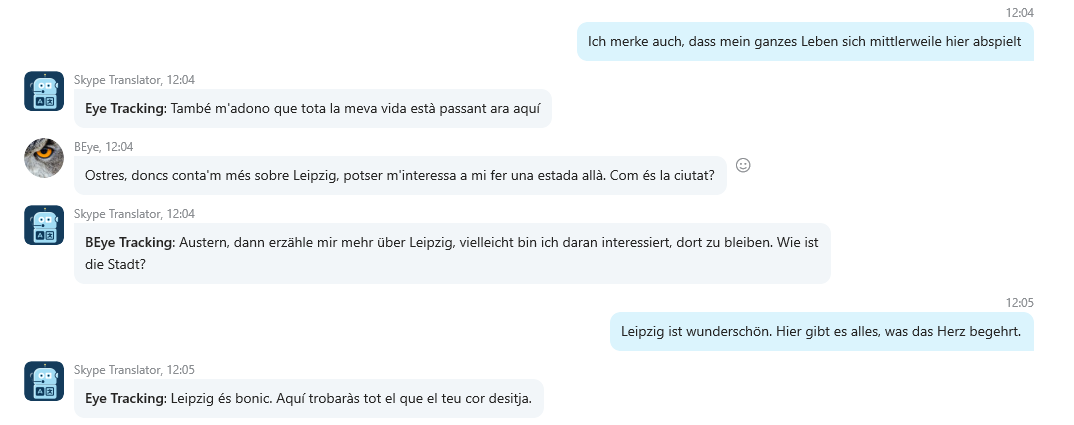
\includegraphics[width=\textwidth]{Figures/Skype/output_ST-ausschnitt.png}
    \caption{Ausgabe des Skype Translators\label{K3:fig:Ausschnitt-Ausgabe-MT-ST}}
\end{figure}

%------------------------------------------------------

Laut Unternehmensdarstellung basiert der Skype Translator auf einem maschinellen Lernprozess und einem proprietären neuronalen MÜ-System. So soll die Qualität der Übersetzung durch häufige Nutzung gesteigert werden, da sich die Präzision der Ausgabe an die wiederholte Eingabe und das Verhalten der Nutzer{\textperiodcentered}innen anpasst.\footnote{Vgl. \url{https://support.skype.com/en/faq/FA34583/skype-translator-privacy-faq}, abgerufen am \datum{}.}

%----------------------------------------------------------------------------------------
% - Es ist zu klären, ob der ST eine maschinelle Verdolmetschung oder Übersetzung ist
%

\subsection{Differenzierung der Technologie}
\label{K3:subsec:DiffTech}

%----------------------------------------------------------------------------------------

Die Betrachtung des Skype Translators als Technologie macht es erforderlich, eine grundlegende Unterscheidung zu treffen. Der Dienst wird zwar als \emph{translator} betitelt, sprich: Texteingaben im Chatfenster werden in Echtzeit dem Kommunikationspartner übersetzt, jedoch bietet er auch die Übersetzung der Gesprächssituation bzw. des Video-Anrufs. Die Wortwahl im vorausgehenden Satz ist dabei bewusst gewählt. Skype selbst begeht diese terminologische Ungenauigkeit.\footnote{Vgl. \url{https://www.skype.com/de/features/skype-translator/}, abgerufen am \datum{}.} Diese Eigenvorstellung macht einen grundsätzlichen Unterschied zwischen der intendierten Nutzer{\textperiodcentered}innenwahrnehmung und der faktischen, wissenschaftlich-technologischen Konzeption des Skype Translators deutlich: Die möglichen Anwender{\textperiodcentered}innen sollen den Skype Translator wohl eher wie einen vollautomatischen Dolmetscher wahrnehmen, der dezent im Hintergrund agiert und verlässliche Ausgaben produziert. So bewirbt Microsoft den Skype Translator auf der Projektwebseite mit dem Anspruch, \glqq Sprachbarrieren in Echtzeit\grqq\footnote{Vgl. \url{https://www.skype.com/de/features/skype-translator/}, abgerufen am \datum{}.\label{K3:footnote:ST-Ad}} überwinden zu können, um sich \glqq nahtlos mit Freunden, Familienmitgliedern, Kunden und Kollegen\grqq{} (s. Fußnote \ref{K3:footnote:ST-Ad}) auszutauschen.

Das wird auch mit Blick auf die Darstellung von Microsofts artverwandtem Projekt \emph{Conversations}\is{Microsoft!Conversations} deutlich.\footnote{Vgl. \url{https://translator.microsoft.com/} bzw. \url{translate.it}, abgerufen am \datum{}.} Conversations beruht auf der gleichen Systemarchitektur wie der Skype Translator und wird (vermutlich) aus den gleichen Ressourcen gespeist. Auf der Webseite des Projektes wird Conversations als dynamisches, interaktives System präsentiert, das dafür sorgt, \glqq dass sich alle willkommen fühlen\grqq{}. Tatsächlich handelt es sich allerdings um eine maschinelle Übersetzung auf Grundlage von statistischen und neuronalen Systemen, die mit einer Spracherkennung und Sprachsynthese kombiniert sind.

\begin{sloppypar}
Ein Unterscheidungsmerkmal zwischen Dolmetschen und Übersetzen ist die Lebensdauer des zu verarbeitenden Textes. Kade weist darauf hin, dass der Ausgangstext beim Dolmetschen flüchtiger Natur sei und meist ausschließlich mündlich vorläge, wohingegen bei der Übersetzung stets schriftlich fixierte Texte aus einer in eine andere Sprache übertragen würden  \citep[34]{kade_zufall_1968}. Dieses Konzept mag heutzutage beinahe als selbstverständlich gelten und den Ausgangspunkt der Dolmetscher- und Übersetzer{\textperiodcentered}innenausbildung darstellen. Für die Funktionsweise des Skype Translators ist der Verweis auf diese Unterscheidung jedoch notwendig, da sich die vorliegende Arbeit ausschließlich dem Textchat widmet. Die Chatnachrichten sind also auch im Nachhinein einsehbar und können bei Bedarf von den am Chat beteiligten Personen erneut gelesen werden -- ganz im Gegenteil zu der flüchtigen Sprachausgabe während des Video- oder Voicechats.
\end{sloppypar}  



%----------------------------------------------------------------------------------------
% - Zu welchem Texttyp ist eigentlich der Output des Skype Translators zuzuordnen? s. Routledge Baker S.223
% - Funktionale Theory des übersetzens, Reiß / Vermeer: Adequatheit & äquivalenz
% - House Model Based Pragmatic Theory (1977--2007), bes. dimensional vs. non-dimensional mismatches
% - Chatbots sollten auch erwähnt werden
%
%
%

%------------------------------------------------------------------------------------------------------

\section{Zum Qualitätsbegriff}
\label{K3:sec:Qualitaet}

%------------------------------------------------------------------------------------------------------

Die vorausgehenden Abschnitte haben den Stand der Technologie grob umrissen. Nun gilt es, die Möglichkeiten zur Evaluation eben dieser aufzuzeigen. Deshalb sei hier zunächst einführend auf den Begriff der \emph{Qualität} geschaut. Der Duden\footnote{Vgl. hierzu \url{https://www.duden.de/rechtschreibung/Qualitaet}, abgerufen am \datum{}.} schreibt dem Wort vier semantische Felder zu: 1) Beschaffenheit, 2) Eigenschaft, 3) Güte und 4) Schach -- wobei letzteres für die vorliegende Arbeit keine Rolle spielt. Die Punkte 1), 2) und 3) haben gemein, dass sie sowohl in Bezug auf Lebewesen als auch auf Materialien verwendet werden. Erwähnenswert ist zudem, dass der Begriff \emph{Qualität} eine Wertsteigerung von neutral zu positiv erfahren hat. Darauf verweist \citet[23]{zech_qualitatsmanagement_2015}, da der lateinische Ursprung ursprünglich nur ein Merkmal oder einen Zustand beschrieb. Erst heutzutage, gerade durch in Verwendung in Kombination mit dem Attributpaar \emph{gut} und \emph{schlecht}, hat sich der Wert des Wortes \emph{Qualität} erhöht \citep[23]{zech_qualitatsmanagement_2015}. Dies ist womöglich auf zweierlei Gründe zurückzuführen: Erstens ist es gegenwärtigen Strategien der Werbebranche geschuldet, Produkte in Qualitätsklassen wie \emph{Standard} und \emph{Premium} zu unterteilen. Zweitens zementiert die Forderung nach Qualitätsmanagement und die Normierung von Prozessen eine gehobene Erwartungshaltung an eben jenen Begriff.

Die Bewertung der Qualität von Übersetzungen, wie sie im Folgenden betrachtet wird, ist zunächst einmal zweierlei: ein sehr breit gefächertes Feld und ein Bereich mit langer Tradition innerhalb der Disziplin. Die Betrachtung des Verhältnisses von Ausgangs- und Zieltext steht nicht erst seit kurzem im Mittelpunkt des Forschungsinteresses. In der Routledge Encyclopedia of Translation wird, ausgehend vom Konzept des \emph{translation quality assessments} (\emph{TQA}), zunächst zwischen verschiedenen Ansätzen und Betrachtungsebenen unterschieden, wobei der Fokus in erster Linie auf der rein menschlichen Tätigkeit liegt. Bei der Qualitätsbewertung wird dort zwischen vier Typen von Ansätzen unterschieden: anekdotische und subjektive, zu denen auch neu-hermeneutische Ansätze zählen, sowie weiterhin antwortorientierte sowie textbasierte Ansätze \citep[222]{baker_routledge_2011}. Ein weiteres kritisches Element bei der Evaluation ist darüber hinaus die Einheit, die betrachtet wird: Werden die einzelnen Wörter des Zieltextes als Bewertungsgrundlage verwendet oder doch die Sätze oder ausschließlich der gesamte Text.

Auch \citet[11]{moorkens_approaches_2018} heben den Stellenwert der Auseinandersetzung mit dem TQA hervor. Neben der vielfältigen Definition des Qualitätsbegriffs gebe es auch in Hinblick auf die Einsatzmöglichkeiten und den Umfang der Evaluation noch zu viele Unterschiede.

\citet[230]{martin_martin_sobre_2010} weist deshalb gleich zu Beginn seines Artikels auf eine der zentralen Herausforderungen hin: Die Tätigkeit des Übersetzens hängt in ihrer Komplexität von vielen Faktoren ab. Diese beeinflussen auch die Bewertung. So gebe es nicht die eine perfekte Übersetzung; es existieren unterschiedliche Schulen; es herrsche kein Konsens über die Bewertungsmethoden \citep[230]{martin_martin_sobre_2010}. Ähnlich fassen auch \citeauthor{moorkens_translation_2018} das Qualitätsmangement im Bereich der Sprachdienstleistung auf. Der Übersetzungsprozess in Verbindung mit der Qualitätsbewertung stellt für sie einen hochkomplexen Vorgang dar, der in den Translationswissenschaften, den Translationstechnologien, unter Sprachdienstleistern und in der Lokalisierungsbranche bislang vielseitig diskutiert wird. Fest steht für die Autoren, dass eine präzise Definition des Qualitätsbegriffs schwierig zu operationalisieren und zu messen ist \citep[2]{moorkens_translation_2018}.

Heutzutage wird sich sowohl manueller als auch automatisierter Verfahren bedient, die in Teilen in international anerkannten Normen fixiert sind. Die folgenden Abschnitte haben somit nicht das Ziel, alle bestehenden Ansätze -- derer es unbestritten viele gibt -- darzustellen. Vielmehr soll es darum gehen, das Gros der einzelnen Theorien herauszuarbeiten und zu präsentieren.

%------------------------------------------------------------------------------------------------------

\subsection{Qualitätsbewertung}
\label{K3:subsec:Qualitaetsbewertung}

%------------------------------------------------------------------------------------------------------

Der folgende Abschnitt ist daher der Qualitätsbewertung gewidmet. Die Qualitätsbewertung stellt bislang den Oberbegriff dar, den es zu differenzieren und in Bezug zum Skype Translator zu setzen gilt. Allein die Erwähnung des Wortes \emph{Qualität} in der Translationswissenschaft impliziert häufig neben der Evaluation auch das Qualitäts- und Risikomanagement \is{Risikomanagement}.

Das wiederum betrifft die Bewertungsmöglichkeiten sowohl für Dolmetsch- als auch Übersetzungstechnologien, in deren Rahmen der Skype Translator sowohl mit einem Angebot für gesprochene als auch geschriebene Kommunikation beworben wird. Erst nach der Ausarbeitung all dieser Faktoren wird es möglich sein, die Wahrnehmung des Skype Translators zu beschreiben, auf der -- in Kombination mit Kapitel \ref{K5} und dem empirischen Teil in Kapitel \ref{K6} -- eine Analyse zum Umgang mit Informationen in einem mehrsprachigen Chat stattfindet.

Das Qualitätsmanagement ist kein Konzept, das exklusiv der Translationswissenschaft vorbehalten ist. Beinahe jeder Wirtschaftszweig hat im Laufe seiner Entwicklung Mechanismen ausgebildet, die ein reibungsloses und effizientes Zusammenspiel aller Beteiligten (z.\,B. Auftraggeber{\textperiodcentered}innen und -nehmer{\textperiodcentered}innen), Prozesse und Objekte (z.\,B. Produkte) gewährleistet. Außerdem ist das Qualitätsmanagement der Evaluation als hierarchisch übergeordnet zu verstehen. Die Evaluation stellt mitunter das zentrale Element für Fortschritt in der Entwicklung -- in diesem Fall in der Entwicklung des Skype Translators -- dar. Durch sie erhalten Forschungsansätze die zwingend notwendige Rückmeldung sowohl über Bereiche, die bereits hohe Qualität aufweisen als auch solchen, die noch einmal überdacht und rekonzipiert werden sollten. 

Das Risikomanagement soll an dieser Stelle weitestgehend ausgespart werden. Der Schwerpunkt des Risikomanagements in der Translationswissenschaft liegt vor allem auf der technischen Dokumentation und der Vermeidung von gravierenden, physischen Unfällen \citep[vgl.\,z.\,B.][]{canfora_risikomanagement_2015, altena_expertenwissen_2014}. Inwiefern oder ob der Skype Translator bei unsachgemäßer Verwendung ein Risiko birgt, bleibt selbstverständlich zu untersuchen. Was nun im Hinblick auf das Übersetzen und Dolmetschen unter Qualitätsmanagement verstanden wird, zeigen die folgenden Abschnitte jeweils für die menschliche Tätigkeit (folgender Abschnitt \ref{K3:subsec:EvaHT}) und maschinelle Verarbeitung (\ref{K3:subsec:EvaMT}, S.\,\pageref{K3:subsec:EvaHT}) auf.



%------------------------------------------------------------------------------------------------------

\subsection{Qualitätsnormen}
\label{K3:subsubsecQualität}

%------------------------------------------------------------------------------------------------------

Eine prominente Rolle nehmen dabei die unterschiedlichen Normen ein, die das Qualitätsmanagement sowie den Begriff Qualität definieren. In der Übersetzungsbranche ist dies die internationale ISO 17100, die generelle Qualitätsanforderungen an die professionelle Übersetzung und den Prozess stellt. \citeauthor{schmitt_translationsqualitat_2007} stellen dem voran die Normenreihe ISO 9000ff. sowie die Definitionen nach ISO 8402 bzw. ISO 9004-2 aus dem Qualitätswesen, nach denen \glqq Qualität (...) also weder etwas Absolutes noch das maximal Machbare, sondern die Erfüllung definierter Erwartungen [ist]\grqq{} \citep[394\psq]{schmitt_translationsqualitat_2007}. In Bezug auf die Arbeitsprozesse in der Übersetzungsbranche versucht DIN 2345, \glqq die Abwicklung von Übersetzungsaufträgen zu vereinfachen und Empfehlungen auszusprechen, zu welchen Punkten Auftraggeber und Übersetzer (durchaus freiwillige) vertragliche Vereinbarungen treffen sollen (...)\grqq{} \citep[396]{schmitt_translationsqualitat_2007}.

%------------------------------------------------------------------------------------------------------

\subsection{Evaluation von menschlichen Übersetzungen}
\label{K3:subsec:EvaHT}

%---------------------------------------------------------------


Die Evaluierung von Übersetzungen beginnt bereits während der Ausbildung, wenn Lehrende die Leistungen der angehenden Sprachmittler{\textperiodcentered}innen beurteilen.
Ein rudimentärer Ansatz ist dabei die manuelle Evaluierung durch professionelle Übersetzer{\textperiodcentered}innen bzw. durch die Kursleitung, indem Ausgangs- und Zieltext miteinander verglichen und anhand einer Skala bewertet werden. Ein zentrales Element ist die Kategorisierung und Gewichtung der Fehler. Die einfache Fehlerannotation mittels Kürzeln dürfte dabei noch aus der Schulzeit bekannt sein: 

	\begin{itemize}
    
	\item \emph{|\,O} für Orthographie
    
    \item \emph{|\,Z} für Zeichensetzung
    
    \item \emph{|\,Präp} für Präposition
    
    \item \emph{Inhalts- und Sinnverschiebungen}
    
    \item usw.
    
	\end{itemize}
    
    
Mitunter kommen auch Zeichen aus dem Umfeld professioneller Korrekturleser{\textperiodcentered}innen und Verleger{\textperiodcentered}innen zum Einsatz, die wie o.\,g. Korrekturmarker sowohl am Seitenrand als auch am betreffenden Zeilenabschnitt angebracht werden. Im Gegensatz zu den Zeichen aus der Schule handelt es sich nicht um Buchstaben, sondern um Symbole wie etwa Kreise oder Pfeile. 

\citet[236]{martin_martin_sobre_2010} stellt jedoch fest, dass bei der Bewertung -- zumindest im akademischen Umfeld -- viel zu stark auf den Fehler fokussiert wird. Positive Aspekte einer Übersetzung finden hingegen kaum Beachtung. Dies ist in Verbindung mit dem Riskomanagement gerade bei Fachübersetzungen nachvollziehbar: Eine gut gestaltete Übersetzung erfüllt schlichtweg ihren Zweck, beispielsweise als Dokumentation oder Bedienungsanleitung eines Produktes. Eine schlechte Übersetzung kommt dem Anspruch nicht nahe und führt im schlimmsten Fall zu einer gesundheitsgefährdenden Verwendung.

In der Praxis kommt bei der Qualitätsbewertung neben dem Bewertungsmaßstab der Textfunktion also noch das potenzielle Risiko für Endnutzer{\textperiodcentered}innen der jeweiligen Übersetzung hinzu. In Kombination können diese beiden Faktoren mit einem Quotienten abgebildet werden, um so die Qualität der Übersetzung auszudrücken. \citet[24]{dalla-zuanna_direkte_2010} beschreibt dieses Vorgehen exemplarisch an den Abläufen in der Übersetzungsabteilung des VW-Konzerns. Die Fehlerkategorien im Beispiel des Autoherstellers sind:

\begin{itemize}

\item Falsche Benennung (\emph{WT}, \emph{Wrong Term})

\item Falsche Bedeutung (\emph{WM}, \emph{Wrong Meaning})

\item Auslassung (\emph{OM}, \emph{Omission})

\item Strukturfehler (\emph{SE}, \emph{Structural Error})

\item Rechtschreibfehler (\emph{SP}, \emph{Misspelling})

\item Interpunktionsfehler (\emph{PE}, \emph{Punctuation Error})

\item Diverses (\emph{ME}, \emph{Miscellaneous Error})

\end{itemize}

Jede dieser Kategorien wird zudem graduell abgebildet durch die Einteilung in mindere und schwere (\emph{minor} und \emph{serious}) Fehler \citep[24]{dalla-zuanna_direkte_2010}. Diese Unterteilung ist keineswegs neu, wie \citet[237]{martin_martin_sobre_2010} mit Verweis auf das kanadische \emph{Translation Bureau} feststellt, das derart schon in den 1980er Jahren vorging. \citet[653]{carstensen_computerlinguistik_2010} merkt an, dass die Bewertung häufig durch mehrere Übersetzer{\textperiodcentered}innen durchgeführt wird, damit sie nicht auf einer einzigen subjektiven Wahrnehmung basiert. In diesem Zusammenhang stellt \citet[3]{williams_translation_2009} fest, dass es zwar einen Bedarf an guten, zufriedenstellenden oder akzeptablen Übersetzungen gibt, die Maßstäbe, mit denen diese Bewertungen festgelegt werden, jedoch national und international undurchsichtig und Gegenstand fortwährender Diskussion sind. Auch \citet[217]{koehn_statistical_2009} und \citet[251]{king_evaluating_1997} weisen auf das Fehlen einer allgemeingültigen Antwort auf die Frage nach der korrekten Bewertungsmethode hin. Ferner ist es \citet[36]{drugan_quality_2013}, die die unübersichtliche Lage innerhalb des akademischen und wirtschaftlichen Bereichs aufgreift. So könnten selbst Theoretiker{\textperiodcentered}innen nicht exakt bestimmen, wie viele Ansätze zur Qualitätsbewertung es überhaupt gäbe \citet[36]{drugan_quality_2013}. Als Hauptgrund führt \citeauthor{drugan_quality_2013} die stark variierenden Bedürfnisse in der Praxis an. Während die Qualitätsbewertung in der Theorie an jeden Einzelfall exemplarisch angepasst werden kann, findet sich in der Praxis eine \glqq huge diversity in real-world needs and requirements\grqq{} \citep[37]{drugan_quality_2013}, was sie an Übersetzungen im medizinischen Bereich exemplifiziert. Dort werden Qualitätsanforderungen nicht nur durch die eigentliche sprachmittlerische Tätigkeit, sondern auch durch die Regularien des Fachgebietes selbst gestellt \citep[37]{drugan_quality_2013}. Aber auch die theoretische Anpassung und Verfeinerung der Modelle störe ein effizientes Qualitätsmanagement.

\citeauthor{williams_translation_2009} schlägt daher vor, sich stärker auf das \emph{translation quality assessment} zu konzentrieren. Der Translationsforschung sei zwar viel daran gelegen, Quellen, Protagonist{\textperiodcentered}innen, Ausgangs- und Zieltexte -- kurzum: das Übersetzen in seiner gesamten Breite -- zu evaluieren, eine einheitliche Festlegung auf Gütegrade habe es bislang jedoch nicht gegeben \citep[4]{williams_translation_2009}.

Die Gründe hierfür sieht \citet[279]{pym_translation_1992} mitunter in der Subjektivität des Forschungsfeldes und in der mangelnden Representativität der durchgeführten Studien. Es sei schlichtweg schwierig, professionelle Sprachmittler{\textperiodcentered}innen als Proband{\textperiodcentered}innen zu rekrutieren, weshalb Studien zur Qualitätsbewertung sich häufig auf Studierende stützten.

Das TQA liefert somit ein Rahmenwerk, innerhalb dessen die Qualität von Übersetzungen eindeutig und objektiv bewertet werden soll. Dabei kann der Ansatz allerdings ebenso variieren wie die Bedeutung des Begriffs \emph{Evaluation}: entweder qualitativ oder quantitativ, diagnostisch, formativ oder summativ. Dieser Ansatz soll es dennoch ermöglichen, allgemein anerkannte Gütekriterien zu benennen \citep[4]{williams_translation_2009}.

\citet[5]{williams_translation_2009} identifiziert acht Faktoren, die es bei der Erstellung eines TQA-Models zu beachten gilt: den/die Übersetzer{\textperiodcentered}in, Stilanforderungen in der Zielsprache, Schwere der Transferfehler, Umfang der Textanalyse, Art der Qualitätsbewertung, Einteilung der Schweregrade von Fehlern, Anzahl an Bewertungsebenen, Eigenanspruch bzw. Zweck der TQA. 

Diesen Aussagen ist jedoch entgegenzusetzen, dass es sehr wohl Normen und Standards gibt, die zumindest europaweit Anwendung finden. Diese enthalten hauptsächlich Empfehlungen und Hinweise zum Qualitäts- und Risikomanagement im Umfeld der menschlichen übersetzerischen Tätigkeit. In ihrem Artikel zu derartigen, übersetzungsbezogenen Normen führen \citet{canfora_im_2015} drei Normen auf, die innerhalb der Branche weit verbreitet sind. Dabei handelt es sich um die sog. \emph{Übersetzungsnorm ISO 17100}, die internationale \emph{Risikomanagementnorm ISO 31000} und die unternehmensbezogene Norm für Qualitätsstandards \emph{DIN EN ISO 9001} \citep[]{canfora_im_2015}.


%------------------------------------------------------------------------------------------------------

% Allerdings ist diese Form der Evaluation zeitaufwändig und kostspielig. Pre- \& Posteditiing miteinbeziehen.


\subsection{Evaluation von maschineller Übersetzung}
\label{K3:subsec:EvaMT}

%------------------------------------------------------------------------------------------------------

Die \emph{Knowledge Base} der \emph{Translation Automation User Society} (\emph{TAUS}) listet mehrere Methoden zur Evaluation von maschineller Übersetzung auf. Die zwei größten Felder dabei sind die Evaluation durch den Menschen und automatisierte Verfahren. Beide Felder unterteilen sich weiterhin in die direkte und indirekte Bewertung. Ferner zählt die TAUS noch die Rückmeldung von Kund{\textperiodcentered}innen und die Evaluation durch die Endnutzer{\textperiodcentered}innen (\emph{community evaluation}) zu den gängigen Methoden \citep[]{translation_automation_user_society_taus_category:evaluation_2017}.

Die Evaluation der MÜ durch den Menschen beruht in erster Linie auf Vergleichen. In dem Fall wird der von der Maschine produzierte Zieltext mit der Referenzübersetzung von menschlichen Übersetzer{\textperiodcentered}innen verglichen. Bei dieser Methode müssen \glqq verschiedene Dimensionen der Übersetzungsqualität getrennt betrachtet (z.\,B.\ grammatische Korrektheit, Flüssigkeit, Übersetzungstreue)\grqq{} \citep[653]{carstensen_computerlinguistik_2010} werden. \citet[218]{koehn_statistical_2009} empfiehlt für die Bewertung mittels Referenzübersetzung den Einsatz von zweisprachigen Gutachter{\textperiodcentered}\linebreak[3]innen, auch wenn dies häufig aufgrund mangelnder Verfügbarkeit nicht möglich ist.

Wie auch schon bei der Bewertung von menschlichen Übersetzungen kann auch in diesem Fall das Verhältnis von Lesbarkeit (\emph{fluency}) und Angemessenheit (\emph{adequacy}) des Zieltextes betrachtet werden \citep[219]{koehn_statistical_2009}. Die Beurteilung erfolgt dabei auf Grundlage einer Skala, die beispielsweise von 0 bis 5 reicht und im Falle der Lesbarkeit von einer einsprachigen Person und im Falle der Angemessenheit von einer bilingualen Person durchgeführt wird \citep[2]{laubli_has_2018}. 

Automatisierte Verfahren bedienen sich hingegen Algorithmen, die die Nähe von Ausgangs- und Zieltext in Relation zu einer Referenzübersetzung abbilden sollen. Auch in diesem Fall stammen die Referenzübersetzungen von einem Menschen. Diese dienen zugleich häufig der Verbesserung der MÜ-Ausgabe \citep[]{lommel_using_2014, laubli_has_2018, ott_analyzing_2018, khayrallah_simulated_2020}. 

\begin{sloppypar}
Die bekanntesten Metriken sind der sog. \emph{Bi-Lingual Evaluation Understudy-Score} ({BLEU-Score})\is{BLEU}\is{Bi-Lingual Evaluation Understudy-Score|see{BLEU}} und seine Weiterentwicklung \emph{METEOR}\is{METEOR}, der \emph{General Text Matcher}\is{General Text Matcher} ({GTM}) sowie die \emph{Translation Error Rate} ({TER})\is{Translation Error Rate}. Weiterhin hat das \emph{US National Institute of Standard and Technology} ({NIST})\is{NIST|see{US National Institute of Standard and Technology}}\is{US National Institute of Standard and Technology} mit dem gleichnamigen Bewertungssystem eine weitverbreitete Methode eingeführt \citep[]{translation_automation_user_society_taus_category:metrics_2017}.
\end{sloppypar}

Der Einsatz automatisierter Verfahren birgt sowohl Vor- als auch Nachteile. Einerseits sind sie für die jeweiligen Unternehmen sowohl in wirtschaftlicher als auch zeitlicher Hinsicht effizienter und aufgrund der algorithmischen Natur auch weitaus konsistenter als eine menschliche Evaluation. Andererseits liefern diese Metriken ausschließlich numerische Werte, die entlang einer entsprechenden Skala interpretiert werden können. Eine individuelle Analyse der Übersetzung bzw. des Übersetzungssystems in puncto Stärken und Schwächen ist hingegen nicht möglich. Daher ist die Forschung in diesem Bereich zu klassifizierenden Ansätzen übergegangen, die zu den bewertenden Systemen Profile und Fehlerklassen erstellt \citep[130\psq]{popovic_language-related_2018}.

Eng mit den Ausführungen der TAUS\is{TAUS|see{Translation Automation User Society}}\is{Translation Automation User Society} verbunden ist die Multidimensionale Qualitätsmetrik\is{Multidimensionale Qualitätsmetrik}\is{Multidimensionale Qualitätsmetrik} (MQM), welche vom Deutschen Forschungszentrum für Künstliche Intelligenz\is{Deutsches Forschungszentrum für Künstliche Intelligenz} entwickelt wird.\footnote{S. hierzu \url{http://www.qt21.eu/mqm-definition/definition-2015-06-16.html}, abgerufen am \datum{}.} Die Metrik steht unter einer Creative-Com\-mons"=Lizenz, welche die Verbreitung unter Namensnennung und ohne Derivate erlaubt.\footnote{S. hierzu \url{https://creativecommons.org/licenses/by-nd/4.0/deed.en_US}, abgerufen am \datum{}.} Damit ermöglicht es diese flexibel konzipierte Metrik, die Qualität von Übersetzungsprojekten zu bewerten und die einzelnen Bereiche der Metrik an die jeweiligen Anforderungen anzupassen \citep[]{lommel_multidimensional_2014}. Die Konzeption einer derart flexiblen Metrik ist zugleich auch der größte Kritikpunkt: Im Gegensatz zu vielen wertbasierten Ansätzen wirkt die MQM zu umfangreich, um kurzfristige Bewertungen vorzunehmen.

%------------------------------------------------------------------------------------------------------

\section{Postediting}
\label{K3:sec:PE}

%------------------------------------------------------------------------------------------------------

Das Postediting\is{Postediting} stellt die nachträgliche Korrektur der rohen MÜ-Ausgabe durch menschliche Übersetzer{\textperiodcentered}innen gemäß festgelegter Richtlinien und Qualitätskriterien dar \citep[197\psq]{obrien_post-editing_2014}. Durch das kontinuierlich wachsende Übersetzungsvolumen nimmt auch der Einsatz von MÜ zu, wodurch sich primär Zeitersparnis erhofft wird. Das wiederum führt professionelle Übersetzer{\textperiodcentered}innen in die Situation, mit Rohübersetzungen arbeiten zu müssen, was bis zu Beginn der 2000er Jahre noch ein gänzlich neues Feld darstellte. Mit der ISO 18587 (2017) besteht mittlerweile jedoch sogar eine Norm, die standardisierte Anforderungen an den Prozess des Posteditierens sowie an die Fähigkeiten der Posteditor{\textperiodcentered}innen stellt.

Übersetzer{\textperiodcentered}innen finden bei der Postedition ein bereits bestehendes textuelles Grüst vor, das sie nachträglich weiterverarbeiten und einen funktionierenden, fehlerfreien Text formen. Verschiedene Studien und Erfahrungsberichte aus der Praxis untersuchen den möglichen Produktivitätsgewinn durch den Einsatz von MÜ und Postediting \citep[]{castilho_reading_2018, macken_quantifying_2020}. Je nach Güte des zur Verfügung stehenden MÜ-Systems kann das Postediting jedoch auch ins Gegenteil schlagen und zeitlichen Mehraufwand sowie höhere Kosten bedeuten. Daher hat sich analog zum Postediting als Nachbearbeitung das sog. Preediting herausgebildet, dessen Ziel die regularisierte, kontrollierte Vorbereitung des Ausgangstexts für die MÜ ist \citep[164]{baker_routledge_2011}.

Das Postediting und die menschliche Übersetzung sind als verschiedene Aufgaben anzusehen. Das ist nicht zuletzt darin begründet, dass die MÜ-Ausgabe andere Merkmale aufweist als die menschliche Übersetzung. Postediting wird in vielen Forschungsbeiträgen deshalb nicht als Art des Korrekturlesens angesehen, sondern strikt davon abgegrenzt.

\citet[8\psq]{massardo_mt_2016} stellen die geläufigste Kategorisierung dieser Tätigkeit vor: das vollständige (\emph{full}) und das leichte (\emph{light}) Postediting. Das vollständige Postediting ist auf ein druck- und veröffentlichungsreifes Endprodukt ausgerichtet. Daher findet die Überprüfung auf nahezu allen Ebenen statt, von der Anpassung von Punktuation, Maßeinheiten und Formaten, über den Umgang mit Eigennamen bis hin zur morpho-syntaktischen Korrektur. Das leichte Postediting hingegen ist auf die generelle Lesbarkeit des Textes ungeachtet des Stils ausgelegt, wobei auch hier bereits auf terminologische Konsistenz und die Vollständigkeit der MÜ-Ausgabe geachtet wird \citep[16\psq]{massardo_mt_2016}.

Die Geschichte des Posteditings ist zudem eng verbunden mit der Entwicklung der MÜ sowie der Evaluation von Übersetzungen. Sie lässt sich an den o.\,g.\ Wegmarken der MÜ (s.\,Abschnitt \ref{K3:sec:Geschichte-Technologie}, S.\,\pageref{K3:sec:Geschichte-Technologie}) nachverfolgen. Eine detaillierte Übersicht präsentiert \citet[293]{garcia_brief_2012}, der das Georgetown-Experiment und den ALPAC-Bericht (S.\,\ref{K3:para:alpac}, S.\,\pageref{K3:para:alpac}) als Ausgangspunkt für die wissenschaftliche und praktische Auseinandersetzung mit nachträglich durch den Menschen bearbeitete MÜ-Ausgaben sieht. Der ALPAC-Bericht führte, wie o.\,g., zu einer drastischen Reduzierung der Forschungsmittel für die MÜ, wodurch auch das Postediting zu\"nachst vernachlässigt wurde. MÜ und Postediting galten zu der Zeit als zu teuer und zeitaufwändig im Vergleich zu menschlichen Übersetzungen \citep[295]{garcia_brief_2012}. Erst in den 1980er Jahren wurde die (Nach-)Bearbeitung der MÜ-Ausgabe aus wirtschaftlicher Sicht für Unternehmen attraktiv \citep[297]{garcia_brief_2012}. Ungefähr zur selben Zeit bildeten sich auch die ersten Richtlinien zum Einsatz von Postediting im Berufsalltag aus (z.\,B.\ TAUS, \cite[]{massardo_mt_2016}), während besonders über die vergangenen zwei Jahrzehnte der Anteil des Posteditings an der akademischen Übersetzer{\textperiodcentered}innenausbildung und am übersetzungswissenschaftlichen Forschungsbetrieb deutlich gesteigert wurde. Auch die überwiegende Mehrheit der professionellen CAT-Tools hat in jüngster Vergangenheit Schnittstellen zur Integration von MÜ erhalten, wodurch dem Postediting im Berufsalltag ein größerer Stellenwert zukommt.


%------------------------------------------------------------------------------------------------------

\section{Usability}
\label{K3:sec:Usability}

%------------------------------------------------------------------------------------------------------

Unter Usability versteht man die Nutzbarkeit oder auch die Nutzer{\textperiodcentered}innen"-freundlichkeit eines Produktes oder einer Software.\footnote{S. hierzu \url{https://www.duden.de/rechtschreibung/Usability}, abgerufen am \datum{}.} Bei der Untersuchung von Usability geht es in erster Linie häufig um die Qualität der Interaktion zwischen Anwender und Produkt. An diesem Punkt wird die Untersuchung der Nutzbarkeit und Nutzer{\textperiodcentered}innen"-freund"-lichkeit bereits in zwei grundlegende Felder unterteilt: Einerseits werden Produkte in der analogen Welt in puncto Ergonomie und Design untersucht. Andererseits bezieht sich das Konzept auf die qualitative Betrachtung von Software, um die es sich auch schwerpunktmäßig im Folgenden handelt.

Die Untersuchung von Nutzer{\textperiodcentered}innenfreundlichkeit ist weiterhin zu differenzieren und auf vielen verschiedenen Ebenen zu verstehen. \citet[]{stapelkamp_screen-_2007} etwa stellt im Umfeld des Screen- bzw. Interfacedesigns die einzelnen Punkte der Projektentwicklung, des Gestaltungsprozesses und der Umsetzung heraus. Ein (Software-)Produkt wird demnach an seiner Form, Funktion und Zielgruppe gemessen.

\begin{quote}
    Da es wünschenswert ist, dass jedes Produkt die Ansprüche und Bedürfnisse seiner Anwender befriedigt und auch die Inbetriebnahme und Nutzung dieser Produkte keine Herausforderung, sondern im Idealfall eine Erleichterung und Bereicherung darstellen sollte, spielt Usability für die Entwicklung von allen Produkten eine entscheidende Rolle. \citep[514]{stapelkamp_screen-_2007}
\end{quote}

Die Forschung zur Nutzbarkeit bzw. der Nutzer{\textperiodcentered}innenfreundlichkeit von maschineller Übersetzung ist nur spärlich ausgeprägt. Der Schwerpunkt des Interesses liegt vor allem auf dem Umgang mit Postediting. In diesem Bereich stützen sich \citeauthor{castilho_evaluating_2016} auf eine Adaption der ISO/TR 16982. Drei wesentliche Aspekte hieraus bilden den Kern der Definition: Effektivität, Effizienz und Zufriedenheit (der Nutzer{\textperiodcentered}innen). \citet[310\psq]{castilho_evaluating_2016} verweisen zwar auf verschiedene Studien in den vergangenen 25 Jahren zum Nutzen von maschinell übersetzten Inhalten. Die meisten von ihnen weisen jedoch normativ-evaluierenden Charakter auf. \citet[79]{castilho_reading_2018} merken in diesem Zusammenhang an, dass trotz eines starken Fokusses auf der Evaluation von MÜ-Qualität Untersuchungen zum Einfluss von maschineller Übersetzung auf Endnutzer{\textperiodcentered}innen bislang unterrepräsentiert sind.

\begin{sloppypar}
Neben dem Einsatz von Eye-Tracking"=Methoden zur Untersuchung des Nutzungsverhaltens und der Interaktivität werden bei Usability-Studien häufig Fragebögen oder Leseverständnistests eingesetzt, die eine subjektiv-individuelle Rückmeldung von den Versuchspersonen ermöglichen sollen. So arbeiten \citet[128]{daems_interactive_2019} mit einem Fragebogen, um die bevorzugte Nutzung von interaktiven SMÜ- oder NMÜ-Systemen beim Postediting zu erheben.
\end{sloppypar}

Der Nutzen einer rohen (eng. \emph{raw}) MÜ-Ausgabe wurde mittels Eye-Tracking"=Methoden erstmals von \citeauthor{doherty_eye_2010} untersucht. Hierzu wurden französchen Muttersprachler{\textperiodcentered}innen einzelne von der MÜ übersetzten Sätze präsentiert. Die Versuchspersonen sollten die Sätze nach ihrer Verständlichkeit bewerten und wurden während der Leseaufgabe von einem Eye"=Tracker erfasst. Die gesammelten Daten wurden mit den Ergebnissen der HTER-Metrik verglichen. \citet[]{doherty_eye_2010} kommen zu dem Schluss, dass der Eye-Tracking"=Einsatz eine wertvolle Ergänzung bei der Evaluation von MÜ sei. Besonders die Möglichkeit, die Interaktion mit der MÜ-Ausgabe zu beobachten, stellt für die Autoren einen besonderen Mehrwert dar.

Unter Rückgriff auf \citeauthor{stapelkamp_screen-_2007} ist es daher notwendig, den Skype Translator besonders unter den folgenden Aspekten zu betrachten: Aus dem Bereich \emph{Form} sind Orientierung, Gestaltungslayout sowie das Screen- und Informationsdesign zu betrachten. Aus dem Bereich \emph{Funktion} fällt dem Interaktions- und Interfacedesign eine wichtige Rolle zu.
 
 

%------------------------------------------------------------------------------------------------------

\section{Zusammenfassung}
\label{K3:sec:Zusammenfassung}

%------------------------------------------------------------------------------------------------------

Das vorausgehende Kapitel hat zunächst die gängigen MÜ-Systeme sowohl historisch als auch funktionell umrissen. Der Schwerpunkt lag auf dem jüngsten Ansatz, der NMÜ, wie sie in Kombination mit der SMÜ mutmaßlich nach allen verfügbaren Quellen für den Skype Translator angewendet wird. Zur genaueren Ein- bzw. Abgrenzung wurde einerseits die Funktion von im professionellen Übersetzungsbereich verwendeten CAT- und CAI-Tools dargestellt. Andererseits wurde genauer auf Dienste für Voice- und Videochats eingegangen, um hierüber eine Brücke zu geläufigen Evaluationsmöglichkeiten von Translationstechnologie zu schlagen. Die Usability spielt in diesem Zusammenhang ebenfalls eine wichtige Rolle, weshalb sie in Verbindung mit dem Postediting den Abschluss dieses Kapitels darstellt.
